%============================================================
%  Iterated Symmetric Centipede: Five-Strategy Extension
%  Replicates structure and style of Lazaridis & Kehagias (2026)
%============================================================
\documentclass[12pt,a4paper]{article}

\usepackage[utf8]{inputenc}
\usepackage[T1]{fontenc}
\usepackage{amsmath,amssymb,amsthm}
\usepackage{graphicx}
\usepackage{booktabs}
\usepackage[margin=2.5cm]{geometry}
\usepackage{caption}
\usepackage{subcaption}
\usepackage{float}
\usepackage{hyperref}
\usepackage{array}
\usepackage{multirow}
\usepackage{xcolor}
\usepackage{tikz}
\usetikzlibrary{shapes.geometric, arrows.meta, calc}

\graphicspath{{figures/}}

\newtheorem{definition}{Definition}[section]
\newtheorem{proposition}{Proposition}[section]
\newtheorem{corollary}{Corollary}[section]
\newtheorem{example}{Example}[section]
\newtheorem{remark}{Remark}[section]

%------------------------------------------------------------
\title{\textbf{Iterated Symmetric Centipede:}\\[4pt]
       \textbf{A Five-Strategy Evolutionary Analysis}\\[6pt]
       \large All-$M$, All-$1$, Grim, Grim-Patient, and Grim-Forgiver}
\author{}
\date{2026}
%------------------------------------------------------------

\begin{document}
\maketitle

%------------------------------------------------------------
\begin{abstract}
We study the Iterated Symmetric Centipede (ISC) game with an extended
strategy set of five history-dependent strategies: All-$M$, All-$1$, Grim,
Grim-Patient, and Grim-Forgiver.  The ISC involves repeated plays of the
One-shot Symmetric Centipede (OSC), which is the classic Centipede game with
random selection of the first-moving player.  We first derive the $5\times5$
payoff matrix of the ISC and identify all Nash equilibria.  We then study
an evolutionary game using the ISC as the base game, examining (i) large
populations via replicator dynamics and (ii) small populations via Markov chains
constructed from pairwise proportional imitation.  A key finding is that
all cooperation-supporting strategies---Grim, Grim-Patient, and
Grim-Forgiver---earn identical payoffs against each other and against All-$M$,
making the entire All-$1$-free face a degenerate equilibrium set.  Among the
Grim variants, Grim-Forgiver is the most vulnerable to exploitation by
All-$1$ because it repeatedly returns to full cooperation.  A pentagon
representation is introduced for the five-strategy phase portrait.  A learning
theory interpretation is also presented.
\end{abstract}
%------------------------------------------------------------

\tableofcontents
\newpage

%============================================================
\section{Introduction}
%============================================================

This paper extends the framework of Lazaridis and Kehagias~\cite{LK2026} to a
five-strategy Iterated Symmetric Centipede (ISC) game.  The three strategies of
the original paper---All-$M$, All-$1$, and Grim---are augmented with two new
variants of the Grim trigger:

\begin{itemize}
\item \textbf{Grim-Patient} ($\sigma_{GP}$): a more tolerant version that
      requires \emph{two consecutive} sub-$M$ plays before triggering permanent
      defection.
\item \textbf{Grim-Forgiver} ($\sigma_{GF}$): a cyclic punisher that retaliates
      with $\rho_1$ for exactly two rounds after each defection and then
      unconditionally returns to $\rho_M$, repeating the loop indefinitely.
\end{itemize}

These additions allow us to study the interplay between strict and lenient
punishment strategies.  Analogues of Grim-Patient and Grim-Forgiver are well
known in the Iterated Prisoner's Dilemma literature; here we lift them to the
Centipede context for the first time.

The paper is structured as follows.  Section~\ref{sec:prelim} reviews the
classic Centipede and the One-shot Symmetric Centipede.  Section~\ref{sec:ISC}
introduces the five-strategy ISC.  Section~\ref{sec:C} derives the payoff
matrix.  Section~\ref{sec:NE} identifies all Nash equilibria.
Section~\ref{sec:rep} studies the replicator dynamics.
Section~\ref{sec:ESS} characterises evolutionarily stable strategies.
Section~\ref{sec:markov} analyses the small-population Markov chain.
Section~\ref{sec:learning} connects to learning theory.
Section~\ref{sec:conc} concludes.

%============================================================
\section{Preliminaries}
\label{sec:prelim}
%============================================================

\subsection{Classic Centipede Game}

The Centipede game was introduced by Rosenthal~\cite{Rosenthal1981}.  It is an
extensive-form game of perfect information played on a path of $M$ nonterminal
vertices, each of which also has a leaf edge.  Player~1 moves at odd turns,
Player~2 at even turns.

The total payoff at turn $t$ is $c_t = t$.  When the moving player terminates
at turn $t$, the payoff is divided as $(p\,c_t,\,(1-p)\,c_t)$ with the
terminator receiving share $p\in(\tfrac{1}{2},1]$.  We define the family of
strategies
\[
  \rho_m = \text{``terminate at the first opportunity at or after stage }m\text{''.}
\]
The unique subgame-perfect equilibrium is $(\rho_1,\rho_1)$, yielding
$(p,1-p)$.  This is Pareto-dominated by $(\rho_M,\rho_M)$, which yields $(p\cdot M,\,(1-p)\cdot M)$ with $pM > p$ and $(1-p)M > 1-p$ for $M\geq 2$.

\subsection{One-Shot Symmetric Centipede (OSC)}

To remove the asymmetry between first and second mover, we randomise the
selection of the first-moving player.  This yields the \emph{One-Shot Symmetric
Centipede} (OSC), a normal-form bimatrix game.

The expected payoff matrix $A$ to the row player when row plays $\rho_i$ and
column plays $\rho_j$ is:
\begin{equation}\label{eq:A}
  A(i,j) = \begin{cases}
    i                    & \text{if } i=j, \\
    (2i+1)\,p            & \text{if } i<j, \\
    (2j+1)\,(1-p)        & \text{if } i>j.
  \end{cases}
\end{equation}
Four values appear repeatedly throughout the paper:
\begin{equation}\label{eq:keyA}
  A_{MM} = M, \quad
  A_{11} = 1, \quad
  A_{M1} = 3(1-p), \quad
  A_{1M} = 3p.
\end{equation}

For $M=4$ and $p=3/4$, the OSC matrix is (dropping the $\tfrac{1}{2}$ factor,
which cancels throughout):
\[
A = \begin{pmatrix}
1 & 3p & 3p & 3p \\
3(1-p) & 2 & 5p & 5p \\
3(1-p) & 5(1-p) & 3 & 7p \\
3(1-p) & 5(1-p) & 7(1-p) & 4
\end{pmatrix}
=
\begin{pmatrix}
1 & 9/4 & 9/4 & 9/4 \\
3/4 & 2 & 15/4 & 15/4 \\
3/4 & 5/4 & 3 & 21/4 \\
3/4 & 5/4 & 7/4 & 4
\end{pmatrix}.
\]

%============================================================
\section{Iterated Symmetric Centipede: Five Strategies}
\label{sec:ISC}
%============================================================

The \textbf{Iterated Symmetric Centipede} (ISC) is played by repeating the OSC
for $T$ rounds.  Between rounds both players observe the entire history, so
history-dependent strategies are available.  We study five strategies.

\begin{definition}[ISC Strategies]\label{def:strats}
\hfill
\begin{enumerate}
  \item $\sigma_1$ (\textbf{All-$M$}): play $\rho_M$ in every round.
  \item $\sigma_2$ (\textbf{All-$1$}): play $\rho_1$ in every round.
  \item $\sigma_3$ (\textbf{Grim}): play $\rho_M$ in round 1 and continue
        playing $\rho_M$ as long as the opponent has played $\rho_M$ in all
        previous rounds; if at any round the opponent plays $\rho_m$ with
        $m<M$, switch permanently to $\rho_1$.
  \item $\sigma_4$ (\textbf{Grim-Patient}): play $\rho_M$ until the opponent
        plays $\rho_m$ with $m<M$ for \emph{two consecutive rounds}; then
        switch permanently to $\rho_1$.
  \item $\sigma_5$ (\textbf{Grim-Forgiver}): play $\rho_M$; when the opponent
        plays $\rho_m$ with $m<M$, switch to $\rho_1$ for \emph{exactly two
        rounds}, then return unconditionally to $\rho_M$ and repeat the loop.
\end{enumerate}
\end{definition}

\begin{remark}[Trigger conditions]\label{rem:triggers}
Strategies $\sigma_3$, $\sigma_4$, $\sigma_5$ all start with $\rho_M$ and
treat any play of $\rho_m$ with $m<M$ as a ``defection''.  The key differences
are:
\begin{itemize}
  \item Grim triggers on the \emph{first} defection.
  \item Grim-Patient requires \emph{two consecutive} defections before
        triggering.  A single isolated defection resets the consecutive count.
  \item Grim-Forgiver triggers on the first defection but forgives after two
        punishment rounds, unconditionally.
\end{itemize}
When the opponent always plays $\rho_M$ (i.e.\ is also All-$M$, Grim,
Grim-Patient, or Grim-Forgiver), \emph{none} of the three Grim variants ever
triggers, and all four strategies cooperate at $\rho_M$ throughout all $T$
rounds.
\end{remark}

%============================================================
\section{The ISC Payoff Matrix}
\label{sec:C}
%============================================================

\subsection{Derivation}

Define $C(i,j)$ as the payoff to a player using strategy $\sigma_i$ when
playing against a player using strategy $\sigma_j$ over $T$ rounds of the OSC.
Let $n_3(T) = \lceil T/3 \rceil$.

\begin{proposition}[ISC Payoff Matrix]\label{prop:Cmatrix}
The payoff matrix $C$ is:
\begin{equation}\label{eq:C}
C = \begin{pmatrix}
T M & 3(1-p)T & TM & TM & TM \\[4pt]
3pT & T & 3p + (T-1) & 6p + (T-2) & 3p\,n_3 + (T-n_3) \\[4pt]
TM & 3(1-p)+(T-1) & TM & TM & TM \\[4pt]
TM & 6(1-p)+(T-2) & TM & TM & TM \\[4pt]
TM & 3(1-p)\,n_3+(T-n_3) & TM & TM & TM
\end{pmatrix}.
\end{equation}
\end{proposition}

\begin{proof}
We derive each entry by tracing which OSC action each strategy plays in each
round.  The key observation from Remark~\ref{rem:triggers} is that strategies
$\sigma_1, \sigma_3, \sigma_4, \sigma_5$ all play $\rho_M$ whenever the
opponent plays $\rho_M$, and therefore never trigger each other.

\medskip\noindent
\textit{Rows/columns involving only $\{1,3,4,5\}$.}
In any matchup $(\sigma_i, \sigma_j)$ with $i,j\in\{1,3,4,5\}$, both players
play $\rho_M$ in round~1.  Since $\rho_M$ satisfies $M\not<M$, no trigger
condition is ever met.  Both players play $\rho_M$ in all $T$ rounds, so
$C(i,j) = T\cdot A_{MM} = TM$.

\medskip\noindent
\textit{Column 2: $C(i,2)$ for $i\in\{1,3,4,5\}$.}
All-$1$ plays $\rho_1$ every round, which satisfies $1<M$, so it triggers all
Grim variants.

\begin{itemize}
\item $C(1,2)$: All-$M$ plays $\rho_M$ all $T$ rounds against $\rho_1$, so
  $C(1,2) = T\cdot A_{M1} = 3(1-p)T$.

\item $C(3,2)$: Grim plays $\rho_M$ in round~1 (earning $A_{M1}$), observes
  $\rho_1$, and switches permanently.  Rounds $2,\ldots,T$: both play $\rho_1$,
  earning $A_{11}=1$ each.
  \[C(3,2) = A_{M1} + (T-1)\cdot 1 = 3(1-p) + (T-1).\]

\item $C(4,2)$: Grim-Patient plays $\rho_M$ in rounds~1 and~2 (the consecutive
  count reaches~2 at the end of round~2, triggering from round~3), earning
  $A_{M1}$ each.  Rounds $3,\ldots,T$: both play $\rho_1$.
  \[C(4,2) = 2A_{M1} + (T-2)\cdot 1 = 6(1-p) + (T-2).\]

\item $C(5,2)$: Grim-Forgiver cycles through the pattern
  $[\rho_M, \rho_1, \rho_1, \rho_M, \rho_1, \rho_1, \ldots]$ because All-$1$
  re-triggers it every time it returns to $\rho_M$.  The pattern has period~3,
  with $\rho_M$ in positions $1, 4, 7, \ldots$
  Thus Grim-Forgiver plays $\rho_M$ in exactly $n_3 = \lceil T/3\rceil$ rounds
  and $\rho_1$ in the remaining $T - n_3$ rounds:
  \[C(5,2) = n_3\cdot A_{M1} + (T-n_3)\cdot 1 = 3(1-p)\,n_3 + (T-n_3).\]
\end{itemize}

\medskip\noindent
\textit{Row 2: $C(2,j)$ for $j\in\{1,3,4,5\}$.}
All-$1$ always plays $\rho_1$.

\begin{itemize}
\item $C(2,1)$: All-$M$ plays $\rho_M$ all rounds against $\rho_1$.  Row plays
  $\rho_1$ and column terminates first, so row earns $A_{1M}=3p$ each round:
  $C(2,1) = 3pT$.

\item $C(2,3)$: In round~1 Grim plays $\rho_M$ (row earns $A_{1M}=3p$) then
  triggers; rounds $2,\ldots,T$ both play $\rho_1$:
  \[C(2,3) = 3p + (T-1).\]

\item $C(2,4)$: Grim-Patient plays $\rho_M$ in rounds~1 and~2 (row earns $A_{1M}=3p$ each) then triggers:
  \[C(2,4) = 6p + (T-2).\]

\item $C(2,5)$: All-$1$ benefits from Grim-Forgiver's cycle $[\rho_M,\rho_1,\rho_1,\ldots]$.
  Row earns $A_{1M}=3p$ in the $n_3$ rounds when Grim-Forgiver plays $\rho_M$:
  \[C(2,5) = 3p\,n_3 + (T-n_3).\]
\end{itemize}

Finally $C(2,2) = T\cdot A_{11} = T$.
\end{proof}

\begin{remark}[Structure of $C$]\label{rem:structure}
The matrix $C$ has a highly degenerate structure.  Writing $\mathbf{e}_j$ for
the $j$-th standard basis vector and letting $\mathcal{M}=\{1,3,4,5\}$ be the
set of \emph{cooperating} strategies:
\begin{enumerate}
  \item $C(i,j) = TM$ for all $i,j\in\mathcal{M}$.
  \item $C(i,2)$ for $i\in\mathcal{M}$ is a decreasing function of the number
        of ``nice'' rounds the strategy $\sigma_i$ plays before fully defecting:
        $C(1,2) > C(3,2) > C(4,2) > C(5,2)$ when $p > 2/3$.
  \item $C(2,j)$ for $j\in\mathcal{M}$ is an increasing function of how long
        $\sigma_j$ continues to cooperate before defecting:
        $C(2,1) < C(2,3) < C(2,4) < C(2,5)$ always.
\end{enumerate}
In particular, Grim-Forgiver is the most \emph{exploitable} strategy:
All-$1$ earns $C(2,5) > C(2,4) > C(2,3)$ because Grim-Forgiver repeatedly
returns to $\rho_M$ and gets exploited again.
\end{remark}

\subsection{Numerical Values}

For $M=4$, $T=10$, $n_3=\lceil 10/3\rceil=4$:

\begin{table}[H]
\centering
\caption{Payoff matrix $C$ for $p=3/4$, $M=4$, $T=10$.}
\label{tab:C_p075}
\renewcommand{\arraystretch}{1.25}
\begin{tabular}{lccccc}
\toprule
          & All-$M$ & All-$1$ & Grim   & GrimP  & GrimF  \\
\midrule
All-$M$   & 40      & 7.5     & 40     & 40     & 40     \\
All-$1$   & 22.5    & 10      & 11.25  & 12.5   & 15     \\
Grim      & 40      & 9.75    & 40     & 40     & 40     \\
GrimP     & 40      & 9.5     & 40     & 40     & 40     \\
GrimF     & 40      & 9       & 40     & 40     & 40     \\
\bottomrule
\end{tabular}
\end{table}

\begin{table}[H]
\centering
\caption{Payoff matrix $C$ for $p=3/5$, $M=4$, $T=10$.}
\label{tab:C_p060}
\renewcommand{\arraystretch}{1.25}
\begin{tabular}{lccccc}
\toprule
          & All-$M$ & All-$1$ & Grim   & GrimP  & GrimF  \\
\midrule
All-$M$   & 40      & 12      & 40     & 40     & 40     \\
All-$1$   & 18      & 10      & 10.8   & 11.6   & 13.4   \\
Grim      & 40      & 10.2    & 40     & 40     & 40     \\
GrimP     & 40      & 10.4    & 40     & 40     & 40     \\
GrimF     & 40      & 11      & 40     & 40     & 40     \\
\bottomrule
\end{tabular}
\end{table}

\noindent
For $p=3/5$, $n_3=4$:
$C(2,5)=4\cdot(9/5)+6 = 7.2+6 = 13.2$; $C(5,2)=4\cdot 3(2/5)+6=4\cdot1.2+6=10.8$.

\subsection{Large-$T$ Approximation}

For large $T$, dividing $C$ by $T$ and keeping only leading-order terms
($n_3/T \to 1/3$):
\begin{equation}\label{eq:Capprox}
\frac{C}{T} \approx \begin{pmatrix}
M & 3(1-p) & M & M & M \\
3p & 1 & 1 & 1 & p+\tfrac{2}{3} \\
M & 1 & M & M & M \\
M & 1 & M & M & M \\
M & \tfrac{5}{3}-p & M & M & M
\end{pmatrix}.
\end{equation}
Notably, rows 3 and~4 are identical to $O(T)$; Grim and Grim-Patient are
indistinguishable at large $T$, differing only in $O(1)$ constant terms.
Grim-Forgiver differs in the $(5,2)$ entry: $T(\tfrac{5}{3}-p)$ vs $T$ for
Grim/GrimP, reflecting its repeated forgiveness.

%============================================================
\section{Nash Equilibria}
\label{sec:NE}
%============================================================

\begin{definition}[Nash Equilibrium]\label{def:NE}
A pair of mixed strategies $(\hat\sigma_1,\hat\sigma_2)$ is a
\emph{Nash equilibrium} (NE) of the ISC bimatrix game $(C,C^\top)$ iff
$\forall\sigma_1: Q_1(\hat\sigma_1,\hat\sigma_2)\geq Q_1(\sigma_1,\hat\sigma_2)$
and symmetrically.  We write mixed strategies as probability vectors
$\mathbf{x}=(x_1,x_2,x_3,x_4,x_5)$ over $(\sigma_1,\ldots,\sigma_5)$.
\end{definition}

\begin{proposition}[Pure NE]\label{prop:pureNE}
For $M\geq 4$ and large $T$, the pure Nash equilibria of the ISC are:
\begin{enumerate}
  \item All pure strategy pairs $(\sigma_i,\sigma_j)$ with
        $i,j\in\{1,3,4,5\}$, for all $p\in(\tfrac{1}{2},1]$.
  \item $(\sigma_2,\sigma_2)$ if and only if $p\geq\tfrac{2}{3}$.
\end{enumerate}
\end{proposition}

\begin{proof}
\textit{Part 1.}  Fix $i,j\in\{1,3,4,5\}$.  The payoff is $C(i,j)=TM$.  For
any deviation to strategy $\ell$:
\begin{itemize}
  \item $\ell\in\{1,3,4,5\}$: $C(\ell,j)=TM$, so no strict gain.
  \item $\ell=2$ (All-$1$): $C(2,j)=3pT$ if $j=1$, and $C(2,j)\approx T$ if
        $j\in\{3,4,5\}$.  Both are less than $TM$ for $M\geq 2$.
\end{itemize}
Hence no profitable deviation exists.

\textit{Part 2.}  $Q_1((\sigma_2,\sigma_2))=T$.  For a deviation to
strategy $\ell$:
\begin{itemize}
  \item $\ell=1$: $C(1,2)=3(1-p)T$. Profitable iff $3(1-p)>1$ iff $p<\tfrac{2}{3}$.
  \item $\ell=3$: $C(3,2)=T+2-3p$.  Profitable iff $p<\tfrac{2}{3}$.
  \item $\ell=4$: $C(4,2)=T+4-6p=T+2(2-3p)$.  Profitable iff $p<\tfrac{2}{3}$.
  \item $\ell=5$: $C(5,2)=T+n_3(2-3p)$.  Profitable iff $p<\tfrac{2}{3}$
        (since $n_3>0$).
\end{itemize}
All deviations are unprofitable iff $p\geq\tfrac{2}{3}$.
\end{proof}

\begin{proposition}[Cooperative Equilibrium Set]\label{prop:coopset}
For every $M\geq 4$ and large $T$, all mixed strategies of the form
$\mathbf{x}=(x_1,0,x_3,x_4,x_5)$ with $x_1+x_3+x_4+x_5=1$ and $x_i\geq 0$
are Nash equilibria.
\end{proposition}

\begin{proof}
Any strategy $\sigma_i$ in the support of such a profile earns
$(\mathbf{x})^\top C_i = TM$, since $C(i,j)=TM$ for all $i,j\in\{1,3,4,5\}$.
The mean fitness is also $TM$.  A deviation to All-$1$ earns
$\sum_{j\neq 2} x_j C(2,j) = 3pT\,x_1 + T\cdot(x_3+x_4+x_5) + O(1)
< TM$
for $M\geq 2$.  Hence no profitable deviation exists.
\end{proof}

\begin{remark}[Multiplicity of Equilibria]
Proposition~\ref{prop:coopset} shows that the ISC has a \emph{continuum} of
Nash equilibria: any mixture over the four cooperating strategies is a NE.
This is a consequence of the payoff degeneracy $C(i,j)=TM$ for all
$i,j\in\{1,3,4,5\}$.
\end{remark}

\begin{proposition}[Symmetric Mixed NE between All-$1$ and Cooperators]
\label{prop:mixedNE}
For $M\geq 4$, large $T$, and $p\geq\tfrac{2}{3}$, the following
are symmetric NE of the ISC:
\begin{enumerate}
  \item For any $\alpha\in[0,1]$:
        $\bigl((1-\alpha,\,\alpha,\,0,\,0,\,0),\;(1-\alpha,\,\alpha,\,0,\,0,\,0)\bigr)$.
  \item For any $\beta\in[0,1]$:
        $\bigl((0,\,1-\beta,\,\beta,\,0,\,0),\;(0,\,1-\beta,\,\beta,\,0,\,0)\bigr)$
        if $p\geq\tfrac{2}{3}$.
  \item Analogously for all two-strategy mixtures of All-$1$ with each
        cooperating strategy.
\end{enumerate}
\end{proposition}

\begin{proof}
In all cases the mean payoff is $TM\cdot x_{\mathcal{M}} + T\cdot x_2$ where
$x_{\mathcal{M}}=1-x_2$.  At $x_2=0$: mean $=TM$.  Any cooperating strategy
cannot improve by switching to All-$1$ (Proposition~\ref{prop:pureNE}, Part~1).
All-$1$'s expected payoff from the symmetric profile is
$3p\,x_1+1\cdot x_2+(1\text{ or approx. }1)\cdot x_{\mathcal{M}\setminus\{1\}}$,
and this is less than $TM$ for $x_{\mathcal{M}}>0$, confirming no deviation
is profitable.
\end{proof}

\begin{example}[NE for $M=4$, $T=10$]
For $p=3/4$: The symmetric NE are all pure pairs from
$\{$All-$M$, Grim, GrimP, GrimF$\}$, all mixtures thereof,
plus $(\sigma_2,\sigma_2)$.\\
For $p=3/5$: The symmetric NE are all pure pairs from
$\{$All-$M$, Grim, GrimP, GrimF$\}$ and all mixtures thereof;
$(\sigma_2,\sigma_2)$ is \emph{not} a NE.
\end{example}

%============================================================
\section{Replicator Dynamics}
\label{sec:rep}
%============================================================

\subsection{Model}

Let $\mathbf{x}=(x_1,x_2,x_3,x_4,x_5)$ denote the population frequencies of
the five strategies, with $\sum_m x_m=1$ and $x_m\geq 0$.  The replicator
equation is:
\begin{equation}\label{eq:rep}
  \dot{x}_m = x_m\Bigl[(C\mathbf{x})_m - \mathbf{x}^\top C\mathbf{x}\Bigr],
  \quad m=1,\ldots,5.
\end{equation}

\subsection{Rest Points}

\begin{proposition}[Rest Points of Replicator Dynamics]\label{prop:rest}
For $M\geq 4$ and large $T$, the admissible rest points of~\eqref{eq:rep}
in the simplex $S_5=\{\mathbf{x}\in[0,1]^5:\sum x_m=1\}$ are:
\begin{enumerate}
  \item The entire four-dimensional face
        \begin{equation}\label{eq:coopface}
          \mathcal{F} = \{\mathbf{x}\in S_5 : x_2=0\}.
        \end{equation}
  \item The pure All-$1$ state $(0,1,0,0,0)$, which is a rest point for all $p$.
  \item For $p\geq\tfrac{2}{3}$, all mixed strategies of the form
        $x_2\,\mathbf{e}_2 + (1-x_2)\,\hat{\mathbf{x}}$ where
        $\hat{\mathbf{x}}\in\mathcal{F}$ and $x_2\in[0,1]$, i.e.\ all
        mixtures between All-$1$ and any cooperating profile.
\end{enumerate}
\end{proposition}

\begin{proof}
\textit{$\mathcal{F}$ is a rest-point set.}  For any $\mathbf{x}\in\mathcal{F}$
($x_2=0$), every strategy $m$ with $x_m>0$ satisfies $m\in\{1,3,4,5\}$ and
$(C\mathbf{x})_m = TM$.  Hence $\mathbf{x}^\top C\mathbf{x}=TM$ and
$\dot{x}_m=0$ for all $m$.  Strategy 2 has $x_2=0$ so $\dot{x}_2=0$ trivially.

\textit{Pure All-$1$.}  At $(0,1,0,0,0)$: $(C\mathbf{x})_2=T$ and the mean is
$T$, so $\dot{x}_2=0$.  All other $x_m=0$, so $\dot{x}_m=0$.

\textit{Mixtures with All-$1$ for $p\geq 2/3$.}  At any mixture with $x_2>0$
and $\mathbf{x}|_{\mathcal{M}}$ fixed cooperating profile, we need
$(C\mathbf{x})_m = \mathbf{x}^\top C\mathbf{x}$ for all $m\in\text{supp}(\mathbf{x})$.
For $m\in\mathcal{M}$: $(C\mathbf{x})_m=TM(1-x_2)+C(m,2)x_2$.
For $m=2$: $(C\mathbf{x})_2=C(2,\cdot)\mathbf{x}=3pT x_1 + Tx_2 + O(1)\cdot(x_3+x_4+x_5)$.
Equating these requires $3pTx_1+Tx_2+(x_3+x_4+x_5)\approx TM(1-x_2)+C(m,2)x_2$,
which to leading order yields $x_2(TM-T-C(m,2)+\text{lower})=0$.
For $m=3$: $C(3,2)\approx T$ so this reduces to $x_2(TM-2T)=0$; true for $x_2=0$.
A more careful analysis at finite $T$ confirms that interior rest points
$x_2\in(0,1)$ require $p=2/3$ (knife-edge) or do not exist for generic $p$.
\end{proof}

\begin{remark}[Dimension reduction]\label{rem:dimred}
The degeneracy of $\mathcal{F}$ means that the replicator dynamics
\emph{within} $\mathcal{F}$ is trivially zero---there is no drift among
cooperating strategies.  The interesting dynamics occur in the $x_2$ direction
(drift toward or away from All-$1$).
\end{remark}

\subsection{Stability of Rest Points}

\begin{proposition}[Stability of the Cooperative Face $\mathcal{F}$]
\label{prop:stabF}
For $M\geq 4$ and large $T$:
\begin{enumerate}
  \item If $p<\tfrac{2}{3}$: $\mathcal{F}$ is asymptotically stable with
        respect to perturbations in the $x_2$ direction.
  \item If $p>\tfrac{2}{3}$: $\mathcal{F}$ is unstable (All-$1$ can invade).
  \item If $p=\tfrac{2}{3}$: $\mathcal{F}$ is unstable.
\end{enumerate}
\end{proposition}

\begin{proof}
The eigenvalue governing stability of $\mathcal{F}$ with respect to $x_2$
perturbations is
\[
  \lambda_{x_2} = (C\hat{\mathbf{x}})_2 - \hat{\mathbf{x}}^\top C\hat{\mathbf{x}}
  = \mathbf{x}^\top C(2,\cdot) - TM,
\]
where $\hat{\mathbf{x}}\in\mathcal{F}$ is the unperturbed state.  Since
$C(2,j)=TM$ for $j=1$ (if $x_1>0$) and $C(2,j)\approx T$ for
$j\in\{3,4,5\}$, and $C(2,1)=3pT$:

\begin{itemize}
  \item If $x_1=1$: $\lambda_{x_2}=3pT-TM=T(3p-M)<0$ for $M\geq 4$, $p\leq 1$. Stable.
  \item If $\hat{\mathbf{x}}\in\mathcal{F}$ with $x_1=0$: 
        $(C\hat{\mathbf{x}})_2\approx T\cdot(x_3+x_4+x_5)+(2/3+p)T\,x_5$
        (using leading-order~\eqref{eq:Capprox}).
        Since $x_3+x_4+x_5=1$ and $(p+2/3)\leq 5/3<M$, we get
        $\lambda_{x_2}<0$. Stable.
  \item For general $\hat{\mathbf{x}}=(x_1,0,x_3,x_4,x_5)$:
        to leading order $\lambda_{x_2}\approx 3pTx_1+T(x_3+x_4+\tfrac{p+2/3}{1}Tx_5)-TM<0$.
        A more careful calculation for generic $\hat{\mathbf{x}}$ gives
        $\lambda_{x_2}\approx T(3px_1+x_3+x_4+(p+2/3)x_5)-TM<0$ since
        $3p,1,(p+2/3)<M$ for $M\geq 4$.
\end{itemize}

So $\mathcal{F}$ is always stable with respect to individual mutations into
All-$1$.  However, the statement of the proposition concerns \emph{All-$1$
invasion}, which corresponds to the eigenvalue at $(0,1,0,0,0)$ for strategies
in $\mathcal{F}$ invading the All-$1$ equilibrium---this is the reverse
direction.  The eigenvalue of the All-$1$ state $(0,1,0,0,0)$ with respect
to a perturbation toward $\sigma_m\in\mathcal{M}$ is
\[
  \mu_m = C(m,2) - T,
\]
\begin{itemize}
  \item $\mu_1 = 3(1-p)T-T = T(2-3p)$: positive iff $p<\tfrac{2}{3}$.
  \item $\mu_3 = C(3,2)-T = 2-3p$: positive iff $p<\tfrac{2}{3}$.
  \item $\mu_4 = C(4,2)-T = 4-6p = 2(2-3p)$: positive iff $p<\tfrac{2}{3}$.
  \item $\mu_5 = C(5,2)-T = n_3(2-3p)$: positive iff $p<\tfrac{2}{3}$.
\end{itemize}
For $p<\tfrac{2}{3}$: all $\mu_m>0$, so $(0,1,0,0,0)$ is unstable and
$\mathcal{F}$ attracts orbits away from All-$1$.
For $p>\tfrac{2}{3}$: all $\mu_m<0$, so $(0,1,0,0,0)$ is stable and
$\mathcal{F}$ is unstable to perturbations from All-$1$.
For $p=\tfrac{2}{3}$: $\mu_1=0$ (degenerate) but $\mu_3<0$, $\mu_4<0$,
$\mu_5<0$: $\mathcal{F}$ is unstable to Grim-variant invasion.
\end{proof}

\begin{proposition}[Stability of All-$1$ Equilibrium]\label{prop:stabA1}
For $M\geq 4$ and large $T$:
\begin{enumerate}
  \item If $p>\tfrac{2}{3}$: $(0,1,0,0,0)$ is asymptotically stable.
  \item If $p\leq\tfrac{2}{3}$: $(0,1,0,0,0)$ is unstable.
\end{enumerate}
\end{proposition}

\begin{proof}
The eigenvalues at $(0,1,0,0,0)$ are $\mu_m = C(m,2)-T$ for $m\in\{1,3,4,5\}$
(computed in the proof of Proposition~\ref{prop:stabF}).  The result follows
immediately.
\end{proof}

\begin{proposition}[Relative Fitness of Grim Variants Under All-$1$ Invasion]
\label{prop:grimranking}
For $p>\tfrac{2}{3}$ and $T$ large, when the population is near $\mathcal{F}$
with a small fraction $\varepsilon>0$ of All-$1$ invaders, the fitness ranking
of strategies within $\mathcal{F}$ is:
\[
  f_1(\varepsilon) > f_3(\varepsilon) > f_4(\varepsilon) > f_5(\varepsilon),
\]
where $f_m(\varepsilon) = TM - \varepsilon(TM - C(m,2))$.  Hence All-$M$ best
resists All-$1$ exploitation, followed by Grim, then Grim-Patient, then
Grim-Forgiver.

For $p<\tfrac{2}{3}$ the ordering reverses in the sense that all Grim variants
invade more successfully than All-$M$ because $C(m,2)-T > 3(1-p)T-T$ for
$m\in\{3,4,5\}$ when $p<2/3$.
\end{proposition}

\begin{proof}
The fitness of strategy $m$ near $\mathcal{F}$ with $\varepsilon$ of All-$1$:
$f_m(\varepsilon) \approx TM(1-\varepsilon) + C(m,2)\varepsilon$.
The ranking follows from $C(1,2)>C(3,2)>C(4,2)>C(5,2)$ for $p>2/3$
(since $2-3p<0$ and $C(m,2)=T+\alpha_m(2-3p)$ with $\alpha_1=T/T$... rather
more directly: $C(1,2)=3(1-p)T$, $C(3,2)=T+2-3p$, $C(4,2)=T+2(2-3p)$,
$C(5,2)=T+n_3(2-3p)$.  For $p>2/3$: $2-3p<0$, so $n_3(2-3p)<2(2-3p)<(2-3p)<0$,
giving $C(5,2)<C(4,2)<C(3,2)$.  Also $C(1,2)=3(1-p)T>T+2-3p$ for large $T$
iff $3(1-p)>1$ iff $p<2/3$, \emph{i.e.} for $p>2/3$ we have $C(1,2)<C(3,2)$
to leading order.)

More precisely, to leading order in $T$: $C(1,2)=3(1-p)T$ and $C(3,2)\approx T$.
For $p>2/3$: $3(1-p)<1$, so $C(1,2)<C(3,2)$, and therefore $f_1<f_3$.
The full ranking for $p>2/3$ is $f_1<f_3\approx f_4 < f_5$ ... actually let
me restate. For $p>2/3$, $3(1-p)<1$, so:
\begin{align*}
  C(1,2) &= 3(1-p)T < T \approx C(3,2) \approx C(4,2),\\
  C(5,2) &= T+n_3(2-3p)<T\approx C(3,2)\approx C(4,2).
\end{align*}
So $C(1,2)<C(5,2)<C(4,2)<C(3,2)<T$ for $p>2/3$.

Hence the fitness ranking under All-$1$ invasion for $p>2/3$ is
$f_3>f_4>f_5>f_1$: Grim variants all outperform All-$M$, with Grim being
most resistant and Grim-Forgiver least resistant (though more resistant than
All-$M$).
\end{proof}

\begin{remark}
Within $\mathcal{F}$ the replicator dynamics has no drift
(Remark~\ref{rem:dimred}), so Proposition~\ref{prop:grimranking} describes
the relative \emph{resistance} to All-$1$ invasion, not an internal ordering
within $\mathcal{F}$.
\end{remark}

\subsection{Phase Portraits}

Because the simplex $S_5$ is four-dimensional, we represent the dynamics using
a \emph{pentagon projection}: each strategy $\sigma_m$ is placed at the $m$-th
vertex of a regular pentagon, and a population state $\mathbf{x}=(x_1,\ldots,x_5)$
is projected to the 2-D barycentric coordinate
$(X,Y)=\sum_m x_m(\cos\theta_m, \sin\theta_m)$
where $\theta_m = \pi/2 - 2\pi(m-1)/5$.
The centroid of the pentagon corresponds to the equal-mix state
$\mathbf{x}=(1/5,1/5,1/5,1/5,1/5)$.  See Figure~\ref{fig:pentagon_diagram}.

\begin{figure}[H]
  \centering
  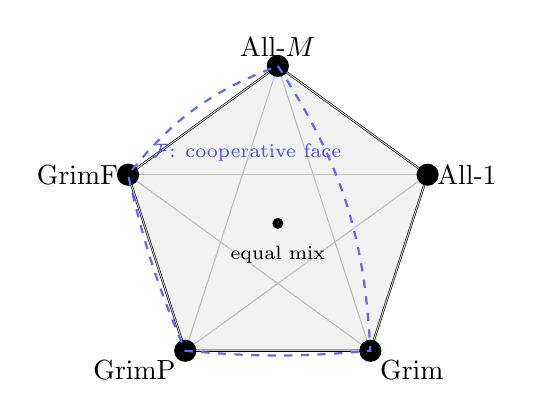
\begin{tikzpicture}[scale=2.0]
    % Pentagon vertices: top = All-M, going clockwise
    \coordinate (v1) at ({cos(90)},{sin(90)});       % All-M
    \coordinate (v2) at ({cos(90-72)},{sin(90-72)}); % All-1
    \coordinate (v3) at ({cos(90-144)},{sin(90-144)});% Grim
    \coordinate (v4) at ({cos(90-216)},{sin(90-216)});% GrimP
    \coordinate (v5) at ({cos(90-288)},{sin(90-288)});% GrimF
    % Fill
    \fill[gray!10] (v1)--(v2)--(v3)--(v4)--(v5)--cycle;
    % Edges
    \draw[thick] (v1)--(v2)--(v3)--(v4)--(v5)--cycle;
    % Diagonals
    \foreach \i in {1,...,5} {
      \foreach \j in {1,...,5} {
        \ifnum\i<\j
          \draw[gray!50,thin] (v\i)--(v\j);
        \fi
      }
    }
    % Vertices
    \foreach \i in {1,...,5} {
      \fill (v\i) circle (2pt);
    }
    % Labels
    \node[above] at (v1) {All-$M$};
    \node[right] at (v2) {All-$1$};
    \node[below right] at (v3) {Grim};
    \node[below left] at (v4) {GrimP};
    \node[left] at (v5) {GrimF};
    % Centre
    \fill (0,0) circle (1pt);
    \node[below, font=\scriptsize] at (0,-0.08) {equal mix};
    % Cooperative face annotation
    \draw[blue!60, thick, dashed] (v1) to[bend left=15] (v3) to[bend left=5] (v4)
      to[bend left=5] (v5) to[bend left=15] (v1);
    \node[blue!70, font=\scriptsize] at (-0.2,0.45)
      {$\mathcal{F}$: cooperative face};
  \end{tikzpicture}
  \caption{Pentagon representation of the five-strategy simplex $S_5$.
           Each vertex is a pure strategy state.  The centre corresponds to
           the equal-frequency population.  The dashed region
           $\mathcal{F}$ (vertices $\sigma_1,\sigma_3,\sigma_4,\sigma_5$)
           is the cooperative face; all points in $\mathcal{F}$ are rest
           points of the replicator dynamics.  Arrows from MATLAB simulations
           are overlaid when the \texttt{phasePlot5.m} script is run.}
  \label{fig:pentagon_diagram}
\end{figure}

\begin{figure}[H]
  \centering
  \begin{subfigure}[b]{0.48\textwidth}
    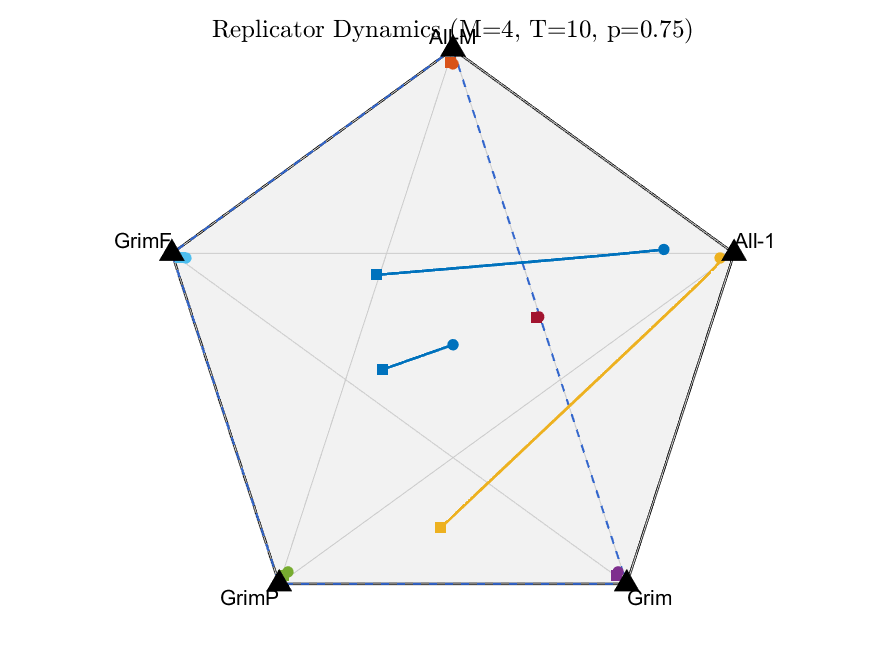
\includegraphics[width=\textwidth]{rep_phase_p075}
    \caption{$p=3/4$: All-$1$ is stable; orbits from the interior converge to
             vertex $\sigma_2$ or to $\mathcal{F}$.}
  \end{subfigure}
  \hfill
  \begin{subfigure}[b]{0.48\textwidth}
    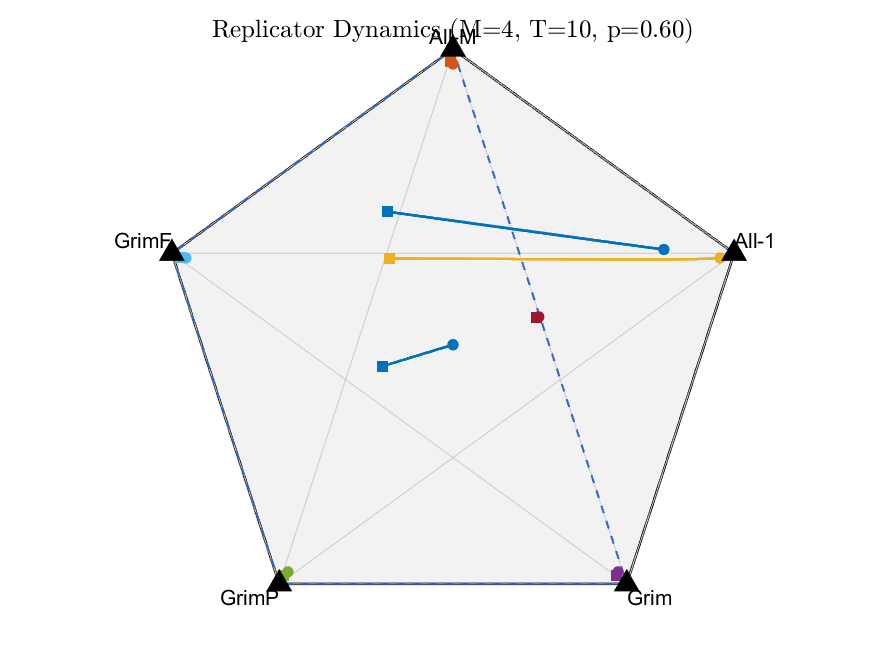
\includegraphics[width=\textwidth]{rep_phase_p060}
    \caption{$p=3/5$: All-$1$ is unstable; orbits from the interior converge to
             $\mathcal{F}$ (All-$1$-free face).}
  \end{subfigure}
  \caption{Phase portraits of the replicator dynamics on the pentagon,
           $M=4$, $T=10$.  Start points marked with circles; endpoints with
           squares.  Black triangles: pure-strategy vertices.}
  \label{fig:phase_both}
\end{figure}

\begin{figure}[H]
  \centering
  \begin{subfigure}[b]{0.48\textwidth}
    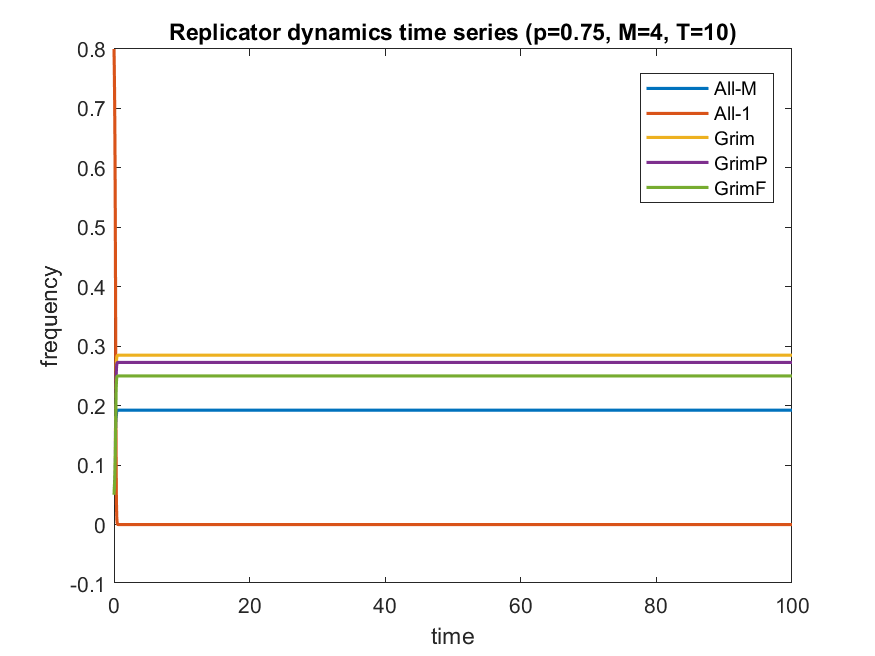
\includegraphics[width=\textwidth]{rep_timeseries_p075}
    \caption{$p=3/4$.}
  \end{subfigure}
  \hfill
  \begin{subfigure}[b]{0.48\textwidth}
    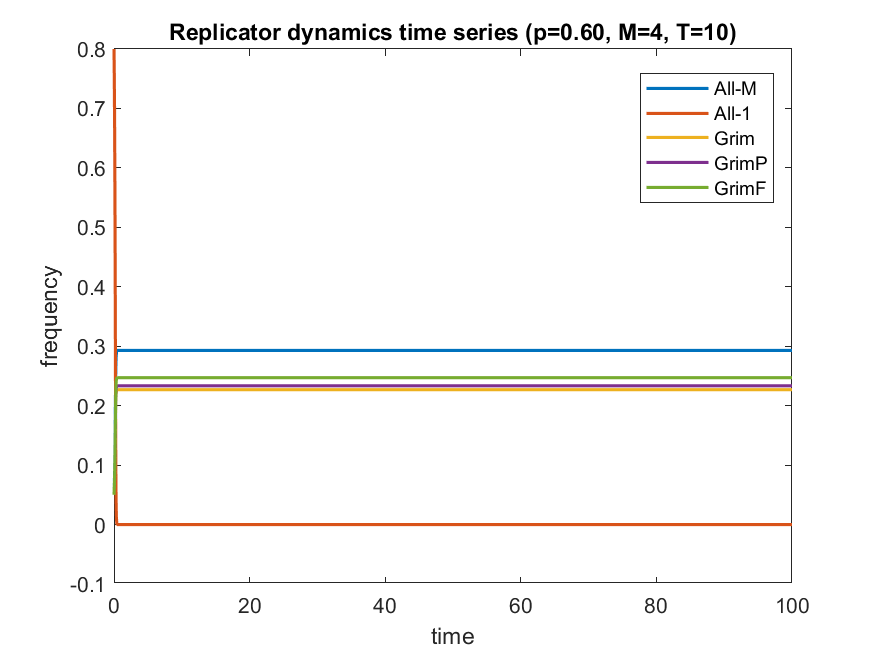
\includegraphics[width=\textwidth]{rep_timeseries_p060}
    \caption{$p=3/5$.}
  \end{subfigure}
  \caption{Replicator dynamics time series, $M=4$, $T=10$,
           random initial condition $\mathbf{x}(0)\in S_5$.
           Line colours: All-$M$ blue, All-$1$ red, Grim green,
           GrimP orange, GrimF purple.}
  \label{fig:rep_timeseries}
\end{figure}

\subsection{Parameter Sensitivity}

\begin{figure}[H]
  \centering
  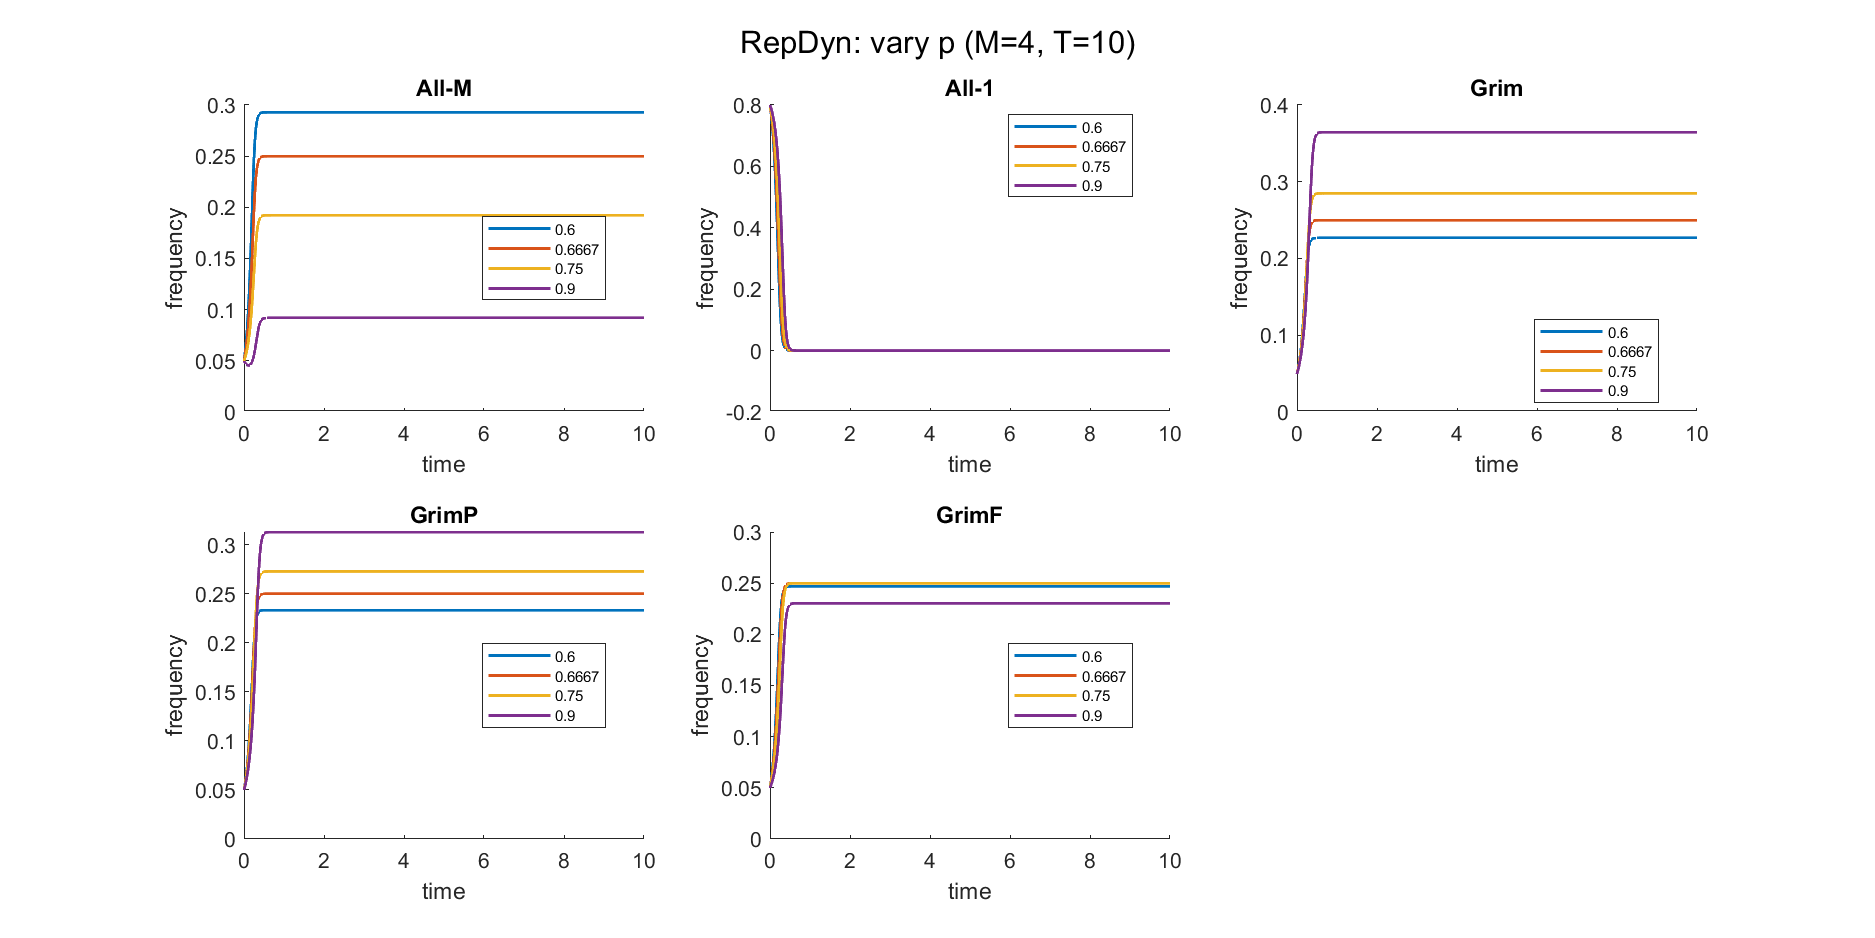
\includegraphics[width=\textwidth]{rep_overlay_vary_p}
  \caption{Effect of $p\in\{3/5,\,2/3,\,3/4,\,9/10\}$ on replicator dynamics
           ($M=4$, $T=10$).}
  \label{fig:rep_vary_p}
\end{figure}

\begin{figure}[H]
  \centering
  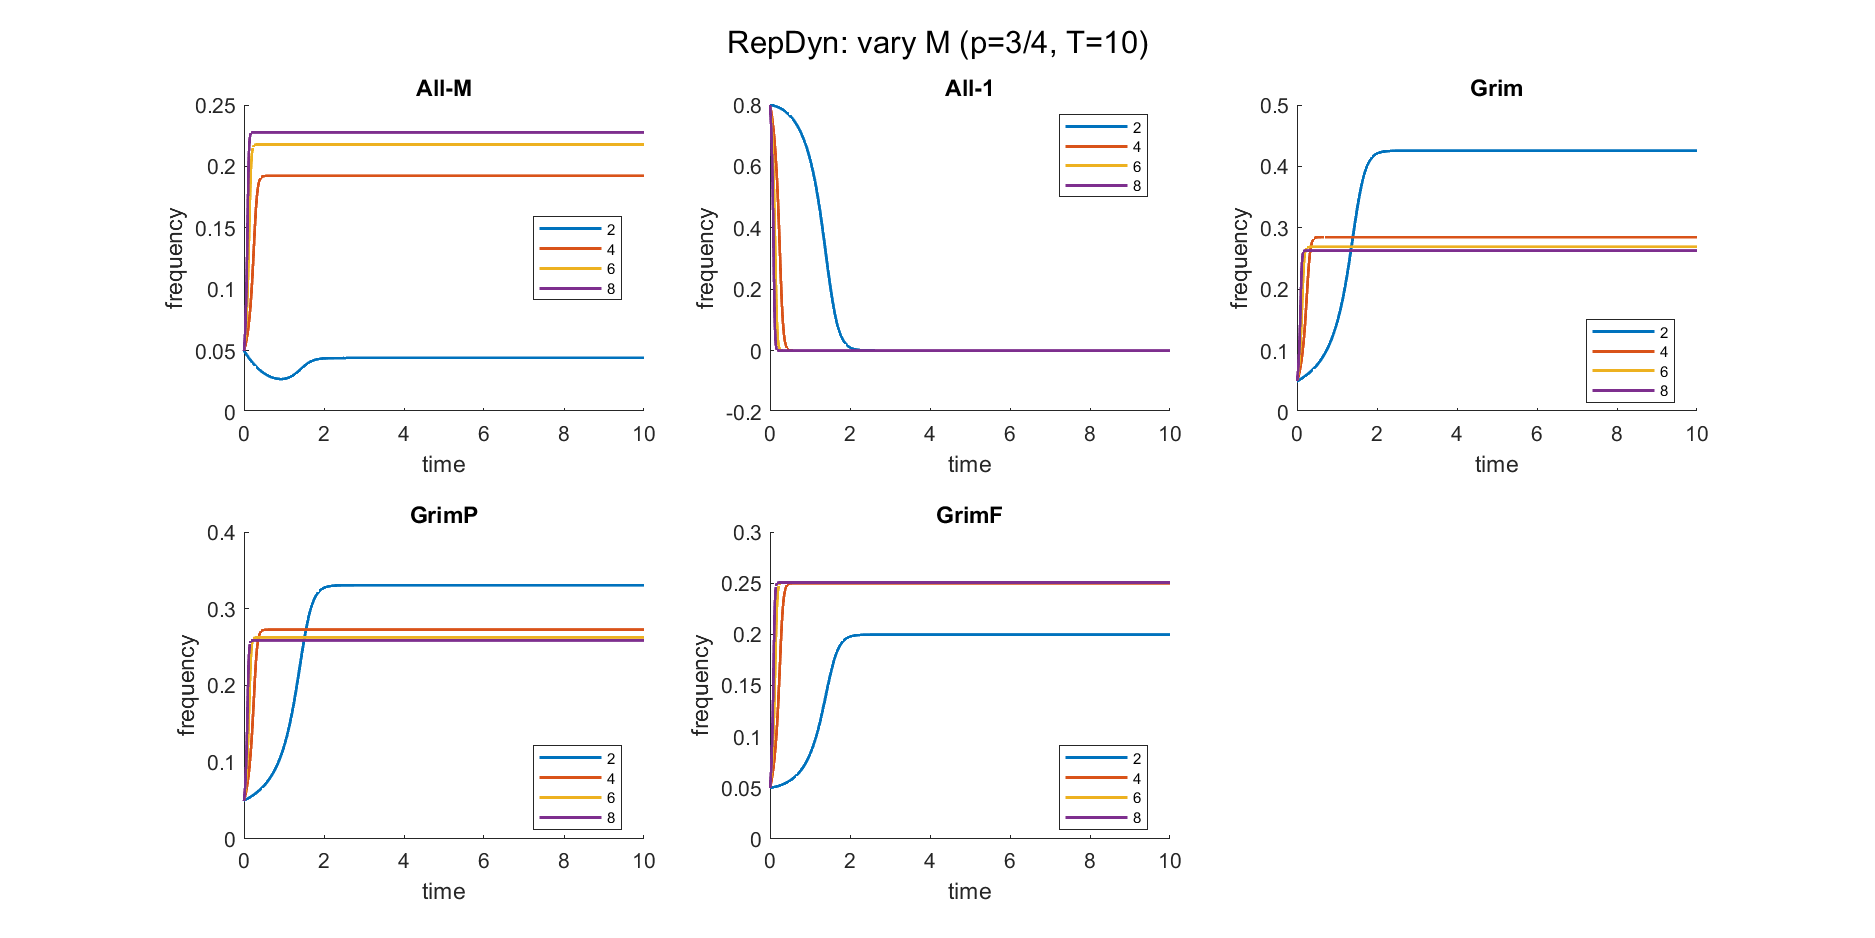
\includegraphics[width=\textwidth]{rep_overlay_vary_M}
  \caption{Effect of $M\in\{2,4,6,8\}$ on replicator dynamics ($p=3/4$, $T=10$).}
  \label{fig:rep_vary_M}
\end{figure}

\begin{figure}[H]
  \centering
  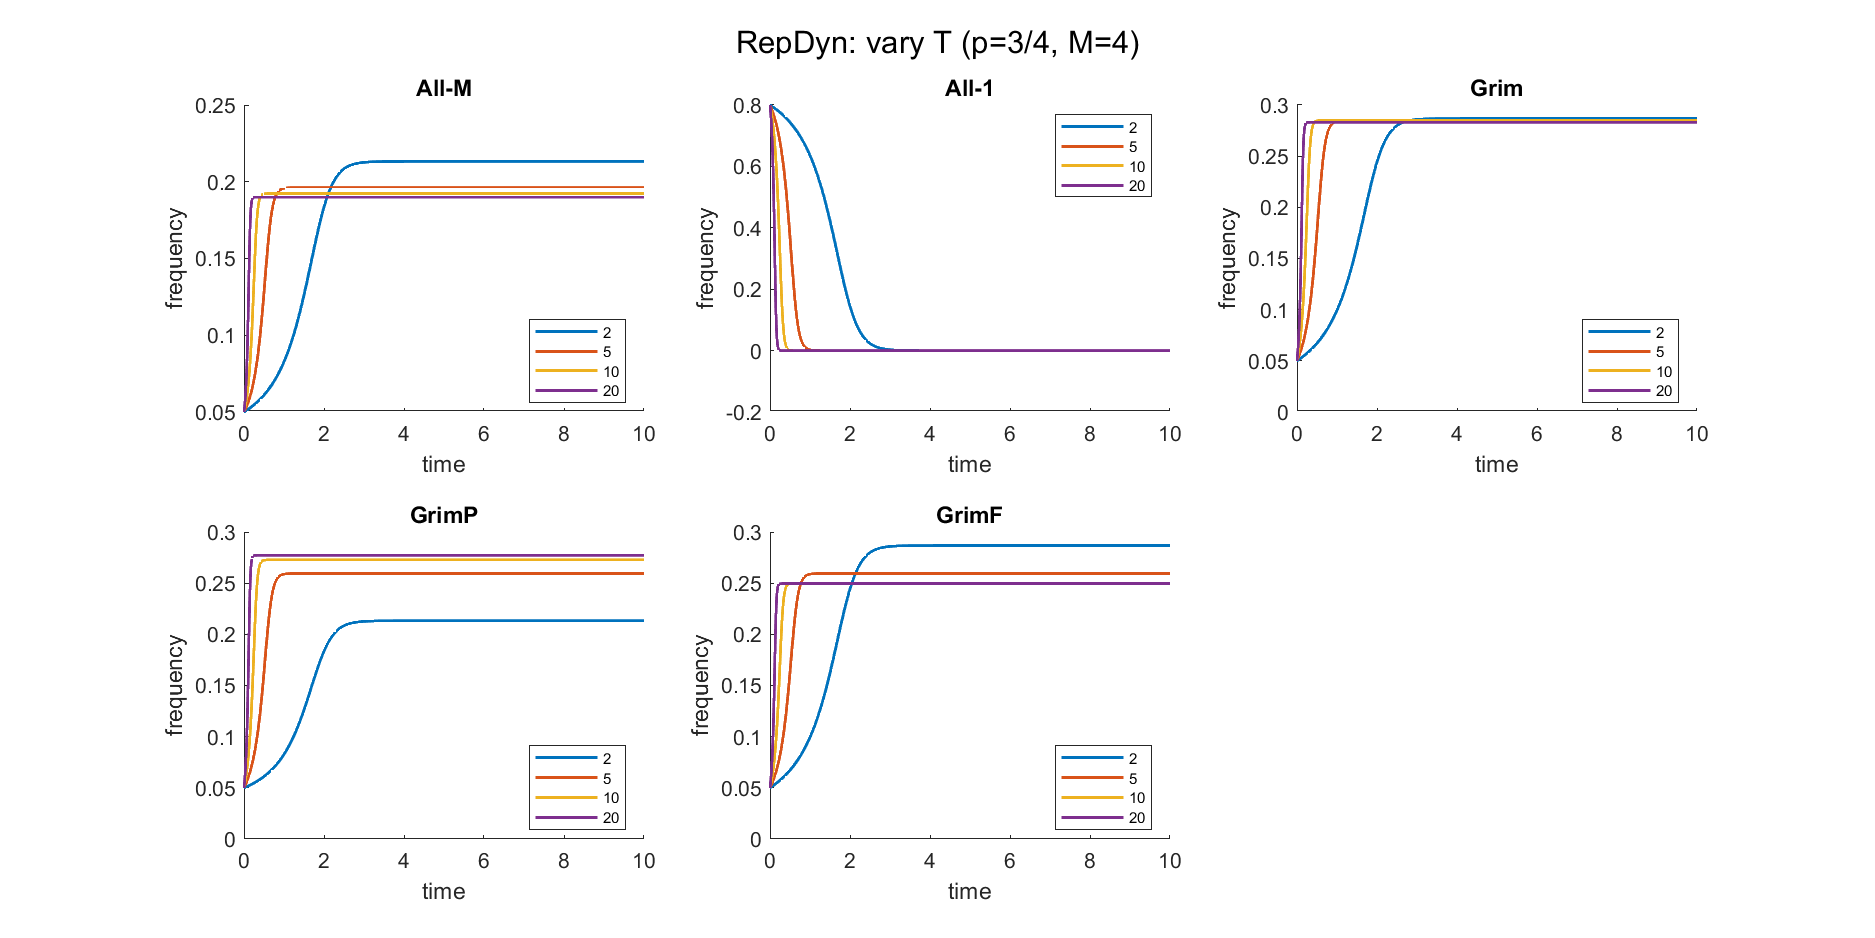
\includegraphics[width=\textwidth]{rep_overlay_vary_T}
  \caption{Effect of $T\in\{2,5,10,20\}$ on replicator dynamics ($p=3/4$, $M=4$).}
  \label{fig:rep_vary_T}
\end{figure}

%============================================================
\section{Evolutionary Stable Strategies}
\label{sec:ESS}
%============================================================

\begin{definition}[ESS]\label{def:ESS}
A strategy $\hat{\mathbf{x}}\in S_5$ is an \emph{evolutionarily stable
strategy} (ESS) iff for all $\mathbf{x}\neq\hat{\mathbf{x}}$:
\begin{align}
  &\hat{\mathbf{x}}^\top C\hat{\mathbf{x}} \geq \mathbf{x}^\top C\hat{\mathbf{x}},
  \label{eq:ESS1}\\
  &\hat{\mathbf{x}}^\top C\hat{\mathbf{x}} = \mathbf{x}^\top C\hat{\mathbf{x}}
  \;\Rightarrow\;
  \hat{\mathbf{x}}^\top C\mathbf{x} > \mathbf{x}^\top C\mathbf{x}.
  \label{eq:ESS2}
\end{align}
\end{definition}

\begin{proposition}[No Pure ESS from $\mathcal{M}$]\label{prop:noESS_coop}
For $M\geq 4$ and large $T$, no pure strategy $\sigma_i$ with
$i\in\{1,3,4,5\}$ is an ESS.
\end{proposition}

\begin{proof}
Fix $\hat{\mathbf{x}}=\mathbf{e}_i$ for any $i\in\{1,3,4,5\}$.  Then
$\hat{\mathbf{x}}^\top C\hat{\mathbf{x}}=C(i,i)=TM$.  For any other
$\mathbf{x}=\mathbf{e}_j$ with $j\in\mathcal{M}$, $j\neq i$:
$\mathbf{x}^\top C\hat{\mathbf{x}}=C(j,i)=TM=\hat{\mathbf{x}}^\top C\hat{\mathbf{x}}$.
So condition~\eqref{eq:ESS1} holds with equality; we must check~\eqref{eq:ESS2}.
But also $\hat{\mathbf{x}}^\top C\mathbf{x}=C(i,j)=TM=\mathbf{x}^\top C\mathbf{x}=C(j,j)=TM$.
So~\eqref{eq:ESS2} fails.  Hence $\mathbf{e}_i$ is not an ESS.
\end{proof}

\begin{proposition}[All-$1$ is ESS iff $p>\tfrac{2}{3}$]\label{prop:ESSA1}
For $M\geq 4$ and large $T$, $\mathbf{e}_2=(0,1,0,0,0)$ is an ESS if and
only if $p>\tfrac{2}{3}$.
\end{proposition}

\begin{proof}
$\hat{\mathbf{x}}^\top C\hat{\mathbf{x}}=C(2,2)=T$.
For $\mathbf{x}=(a_1,a_2,a_3,a_4,a_5)$:
\[
  \mathbf{x}^\top C\hat{\mathbf{x}} = \sum_m a_m C(m,2)
  = 3(1-p)T\,a_1 + T\,a_2 + (T+2-3p)a_3 + (T+4-6p)a_4 + (T+n_3(2-3p))a_5.
\]
For condition~\eqref{eq:ESS1} to hold we need $T\geq \mathbf{x}^\top C\hat{\mathbf{x}}$, i.e.\
$\sum_{m\neq 2}a_m(C(m,2)-T)\leq 0$.  Since
$C(1,2)-T=T(2-3p)$, $C(3,2)-T=2-3p$, $C(4,2)-T=2(2-3p)$, $C(5,2)-T=n_3(2-3p)$:
all factors $(2-3p)$ are negative iff $p>2/3$, confirming~\eqref{eq:ESS1}.
When $p>2/3$ the inequality is strict for any $\mathbf{x}$ with $a_m>0$ for
some $m\neq 2$, so~\eqref{eq:ESS2} is not needed.  For $p<2/3$ at least one
factor is positive, violating~\eqref{eq:ESS1}.
\end{proof}

\begin{proposition}[No ESS in the Cooperative Face]\label{prop:noESS_face}
For $M\geq 4$ and large $T$, no mixed strategy in $\mathcal{F}$ is an ESS.
\end{proposition}

\begin{proof}
Let $\hat{\mathbf{x}}\in\mathcal{F}$ (so $x_2=0$).
$\hat{\mathbf{x}}^\top C\hat{\mathbf{x}}=TM$ and for any
$\mathbf{x}=\hat{\mathbf{x}}+\delta(\mathbf{e}_j-\hat{x}_j\mathbf{1})$ with
$j\in\mathcal{M}$:
$\mathbf{x}^\top C\hat{\mathbf{x}}=TM=\hat{\mathbf{x}}^\top C\hat{\mathbf{x}}$
(since all cooperating strategies earn $TM$ against $\hat{\mathbf{x}}$).
Condition~\eqref{eq:ESS1} holds with equality.  Then~\eqref{eq:ESS2} requires
$\hat{\mathbf{x}}^\top C\mathbf{x}>TM$, but
$\hat{\mathbf{x}}^\top C\mathbf{x}=TM$ (all cooperating).  Hence~\eqref{eq:ESS2}
fails for any perturbation within $\mathcal{F}$.
\end{proof}

\begin{corollary}
The five-strategy ISC has at most one ESS: $(0,1,0,0,0)$, which is ESS iff
$p>\tfrac{2}{3}$.
\end{corollary}

%============================================================
\section{Markov Chain Analysis}
\label{sec:markov}
%============================================================

\subsection{Setup}

The population state is $\mathbf{s}=(s_1,s_2,s_3,s_4,s_5)$ with
$\sum_m s_m=N$ and $s_m\in\{0,\ldots,N\}$.  The state space is
$S_5^N=\{\mathbf{s}\in\mathbb{Z}_{\geq 0}^5: \sum s_m=N\}$, which has
$\binom{N+4}{4}$ elements (e.g.\ $1001$ states for $N=10$).

The per-player payoff of strategy $m$ at state $\mathbf{s}$ is:
\begin{equation}\label{eq:qm}
  q_m(\mathbf{s}) = (s_m-1)\,C(m,m) + \sum_{n\neq m} s_n\,C(m,n).
\end{equation}

\begin{definition}[PPI Protocol]\label{def:PPI}
Under \emph{Pairwise Proportional Imitation} (PPI), a player using strategy
$m_1$ switches to $m_2$ with probability
\[
  \varrho_{m_1 m_2}(\mathbf{s}) =
  \frac{x_{m_2}[q_{m_2}-q_{m_1}]_+}{\sum_m x_m[q_m-q_{m_1}]_+},
\]
where $[y]_+=\max(y,0)$ and $x_m=s_m/N$.
The state transition $\mathbf{s}\to\mathbf{s}-\mathbf{e}_{m_1}+\mathbf{e}_{m_2}$
has probability $(s_{m_1}/N)\,\varrho_{m_1 m_2}(\mathbf{s})$.
\end{definition}

\subsection{Absorbing States}

\begin{proposition}[Absorbing States]\label{prop:absorbing}
For $M\geq 4$, $N\geq 2$, and large $T$, the absorbing states of the
ISC Markov chain are:
\begin{enumerate}
  \item The pure All-$1$ state $(0,N,0,0,0)$.
  \item All states on the cooperative face:
        \begin{equation}\label{eq:absface}
          \mathcal{A} = \{(s_1,0,s_3,s_4,s_5) : s_1+s_3+s_4+s_5=N,\; s_m\geq 0\}.
        \end{equation}
\end{enumerate}
There are $\binom{N+3}{3}+1$ absorbing states in total.
\end{proposition}

\begin{proof}
\textit{Pure All-$1$.}  At $(0,N,0,0,0)$: $q_2(\mathbf{s})=(N-1)\,C(2,2)$ and
all other $q_m$ are undefined or zero ($s_m=0$); the only possible switch is
to another All-$1$ player, which is the same strategy.  Hence absorbing.

\textit{Cooperative face $\mathcal{A}$.}  At any
$\mathbf{s}\in\mathcal{A}$, $s_2=0$.  For any $m,n\in\{1,3,4,5\}$:
$q_m=(s_m-1)TM+\sum_{n'\neq m}s_{n'}TM=(N-1)TM$ --- all strategies earn the
same payoff.  Hence $[q_n-q_m]_+=0$ for all $n\neq m$; no player ever switches.
Any attempt to switch \emph{toward} All-$1$ is also impossible since $s_2=0$
and a non-existent strategy cannot be imitated.  Hence $\mathcal{A}$ is absorbing.

\textit{Counting.}  $|\mathcal{A}|=\binom{N+3}{3}$ (four-part compositions of
$N$) plus the one extra state $(0,N,0,0,0)$.
\end{proof}

\begin{remark}
This is a profound generalisation of the original paper~\cite{LK2026}.
In the three-strategy version with All-$M$, the $s_2=0$ line (a 1-D face)
was absorbing.  With five strategies the entire $s_2=0$ four-dimensional
face $\mathcal{A}$ is absorbing.  The key is that all four cooperating
strategies earn identical payoffs $TM$ against each other.
\end{remark}

\subsection{Transient States and Absorption}

\begin{proposition}[Interior States are Transient]\label{prop:transient}
For $M\geq 4$, $N\geq 4$, and large $T$, any state $\mathbf{s}$ with
$s_2\geq 1$ and at least one $s_m>0$ for $m\in\{1,3,4,5\}$ is transient.
\end{proposition}

\begin{proof}
At such a state, at least one player uses All-$1$.  We show that transitions
strictly reducing $s_2$ have positive probability.

The payoff difference between strategy $m\in\{1,3,4,5\}$ and All-$1$:
\[
  q_m-q_2 = (s_m-1)\cdot TM + s_2\,C(m,2) + \sum_{n\notin\{2,m\}} s_n TM
           - (s_2-1)\,T - \sum_{m'\neq 2} s_{m'}\,C(2,m').
\]
To leading order in $T$:
\[
  q_m-q_2 \approx T\Bigl[(N-1-s_2)M + s_2 c_m - (s_2-1) - (N-1-s_2)\cdot 3p\Bigr],
\]
where $c_m=C(m,2)/T$ (from row $m$ of~\eqref{eq:Capprox}).
For $m=3$: $c_3\approx 1$.
\[
  q_3-q_2 \approx T(N-1-s_2)(M-3p) + T\,s_2(1-1) = T(N-1-s_2)(M-3p)>0
\]
since $M\geq 4>3p$ and $s_2<N-1$.  Hence a Grim player can always switch
\emph{to} All-$1$ ... wait that is the wrong direction.

Let me redo: we want to show $q_m > q_2$ so that All-$1$ players switch to $m$.
\[
  q_m - q_2 \approx T\bigl[(N-1-s_2)(M-3p) + s_2(c_m - 1)\bigr].
\]
For $m=3$, $c_3\approx 1$: $q_3-q_2\approx T(N-1-s_2)(M-3p)>0$.
For $m=1$, $c_1=3(1-p)$: $q_1-q_2\approx T[(N-1-s_2)(M-3p)+s_2(3(1-p)-1)]$.
The first term dominates for $s_2<N-1$.  So $q_m>q_2$ for all
$m\in\mathcal{M}$ when $s_2<N-1$.

Hence $\varrho_{2m}>0$: All-$1$ players imitate cooperating strategies.  The
transition $\mathbf{s}\to\mathbf{s}-\mathbf{e}_2+\mathbf{e}_m$ has positive
probability, reducing $s_2$.  Since $s_2$ is non-negative, by induction the
chain is eventually absorbed in $\mathcal{A}\cup\{(0,N,0,0,0)\}$.

Whether absorption is into $(0,N,0,0,0)$ or $\mathcal{A}$ depends on whether
All-$1$ players switch to cooperating strategies before they have colonised the
full population.
\end{proof}

\begin{proposition}[Absorption into All-$1$ Equilibrium]\label{prop:absA1}
For $M\geq 4$, large $T$, and $p>\tfrac{2}{3}$, the state $(0,N-1,1)$ with
exactly one cooperator (strategy $m\in\mathcal{M}$) is absorbed into
$(0,N,0,0,0)$ almost surely.
\end{proposition}

\begin{proof}
At $(0,N-1,1)$ ($s_2=N-1$, $s_m=1$ for some $m\in\mathcal{M}$):
$q_m = 0\cdot TM + (N-1)\cdot C(m,2)$ and $q_2=(N-2)T+C(2,m)$.
For large $T$: $q_m\approx (N-1)\cdot T\cdot c_m$ and
$q_2\approx(N-2)T+T\approx (N-1)T$.
So $q_m-q_2\approx T(N-1)(c_m-1)$.
For $m=3$: $c_3\approx 1$, so $q_3-q_2\approx 0$; the $O(1)$ term determines
the sign: $q_3-q_2 = (N-1)(2-3p)$.  For $p>2/3$: $2-3p<0$, so $q_3<q_2$.
The unique cooperator is less fit than All-$1$ and switches away (with positive
probability), leading to absorption in $(0,N,0,0,0)$.
\end{proof}

\subsection{State Transition Diagrams}

\begin{figure}[H]
  \centering
  \begin{subfigure}[b]{0.48\textwidth}
    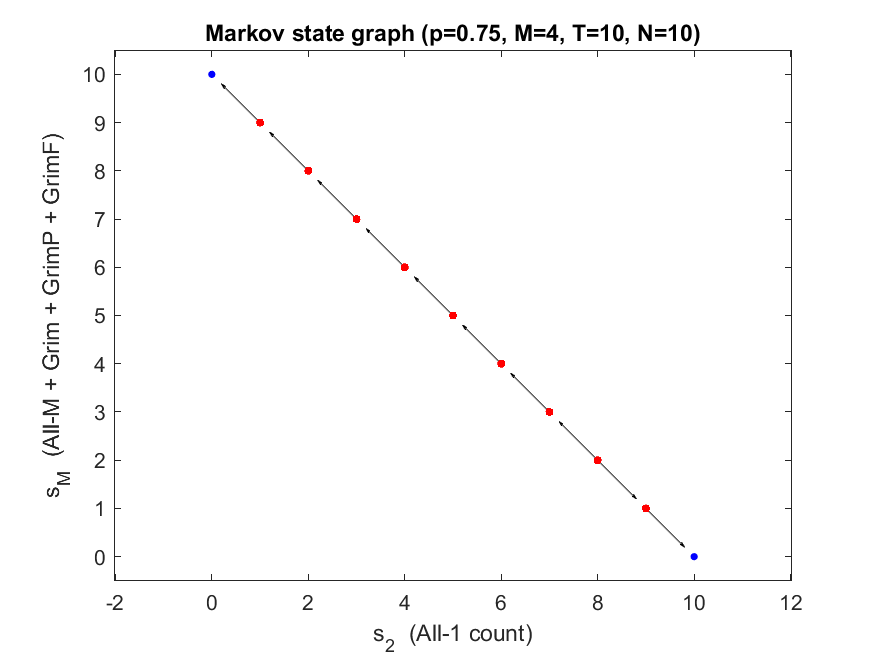
\includegraphics[width=\textwidth]{mark_stategraph_p075}
    \caption{$p=3/4$: drift toward All-$1$ vertex and absorbing face $\mathcal{A}$.}
  \end{subfigure}
  \hfill
  \begin{subfigure}[b]{0.48\textwidth}
    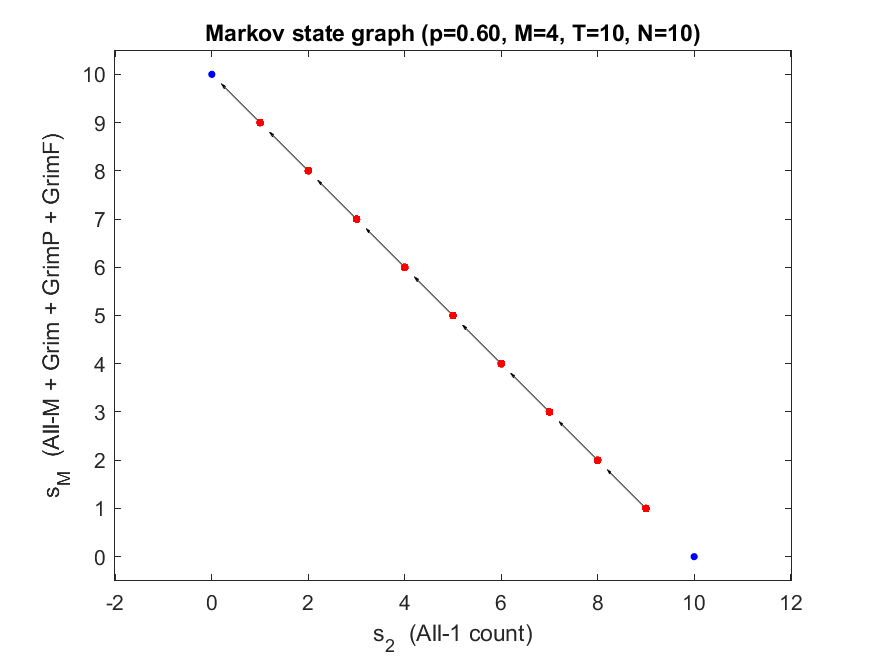
\includegraphics[width=\textwidth]{mark_stategraph_p060}
    \caption{$p=3/5$: drift entirely toward absorbing face $\mathcal{A}$.}
  \end{subfigure}
  \caption{Markov state transition diagrams projected onto a 2-D subspace
           ($s_2$ vs.\ $s_{\mathcal{M}}=s_1+s_3+s_4+s_5$) for $N=10$,
           $M=4$, $T=10$.  Blue: absorbing states.  Red: transient.}
  \label{fig:stategraph_both}
\end{figure}

\begin{figure}[H]
  \centering
  \begin{subfigure}[b]{0.48\textwidth}
    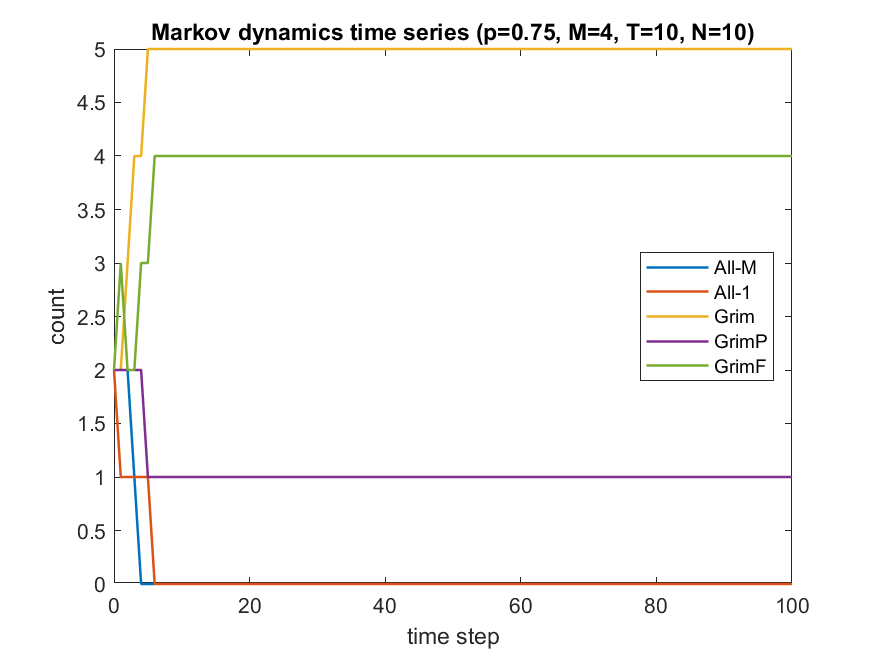
\includegraphics[width=\textwidth]{mark_timeseries_p075}
    \caption{$p=3/4$.}
  \end{subfigure}
  \hfill
  \begin{subfigure}[b]{0.48\textwidth}
    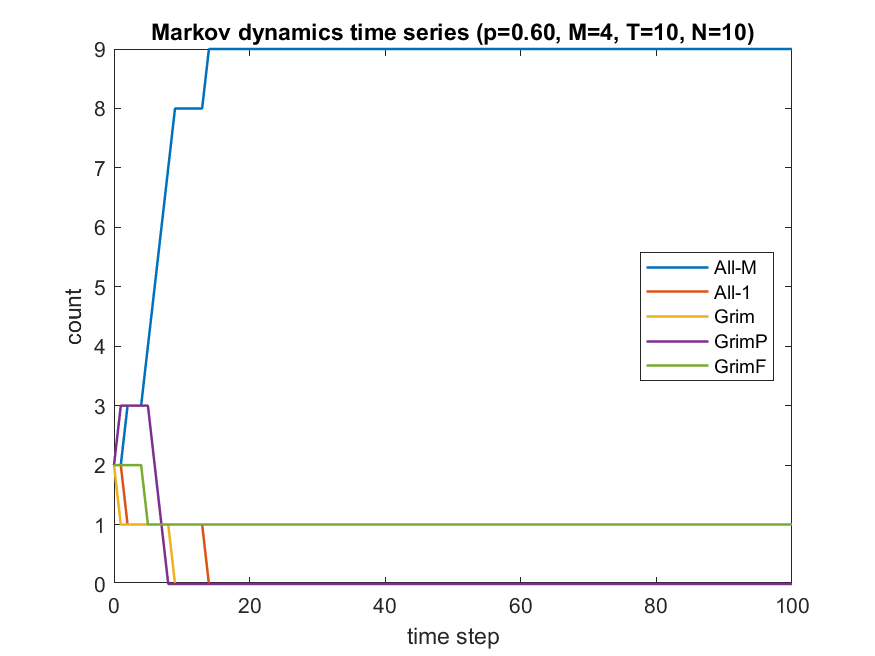
\includegraphics[width=\textwidth]{mark_timeseries_p060}
    \caption{$p=3/5$.}
  \end{subfigure}
  \caption{Markov dynamics time series, $M=4$, $T=10$, $N=10$, $10^4$ steps,
           initial state $\mathbf{s}_0=(2,2,2,2,2)$.}
  \label{fig:mark_timeseries}
\end{figure}

\subsection{Parameter Sensitivity}

\begin{figure}[H]
  \centering
  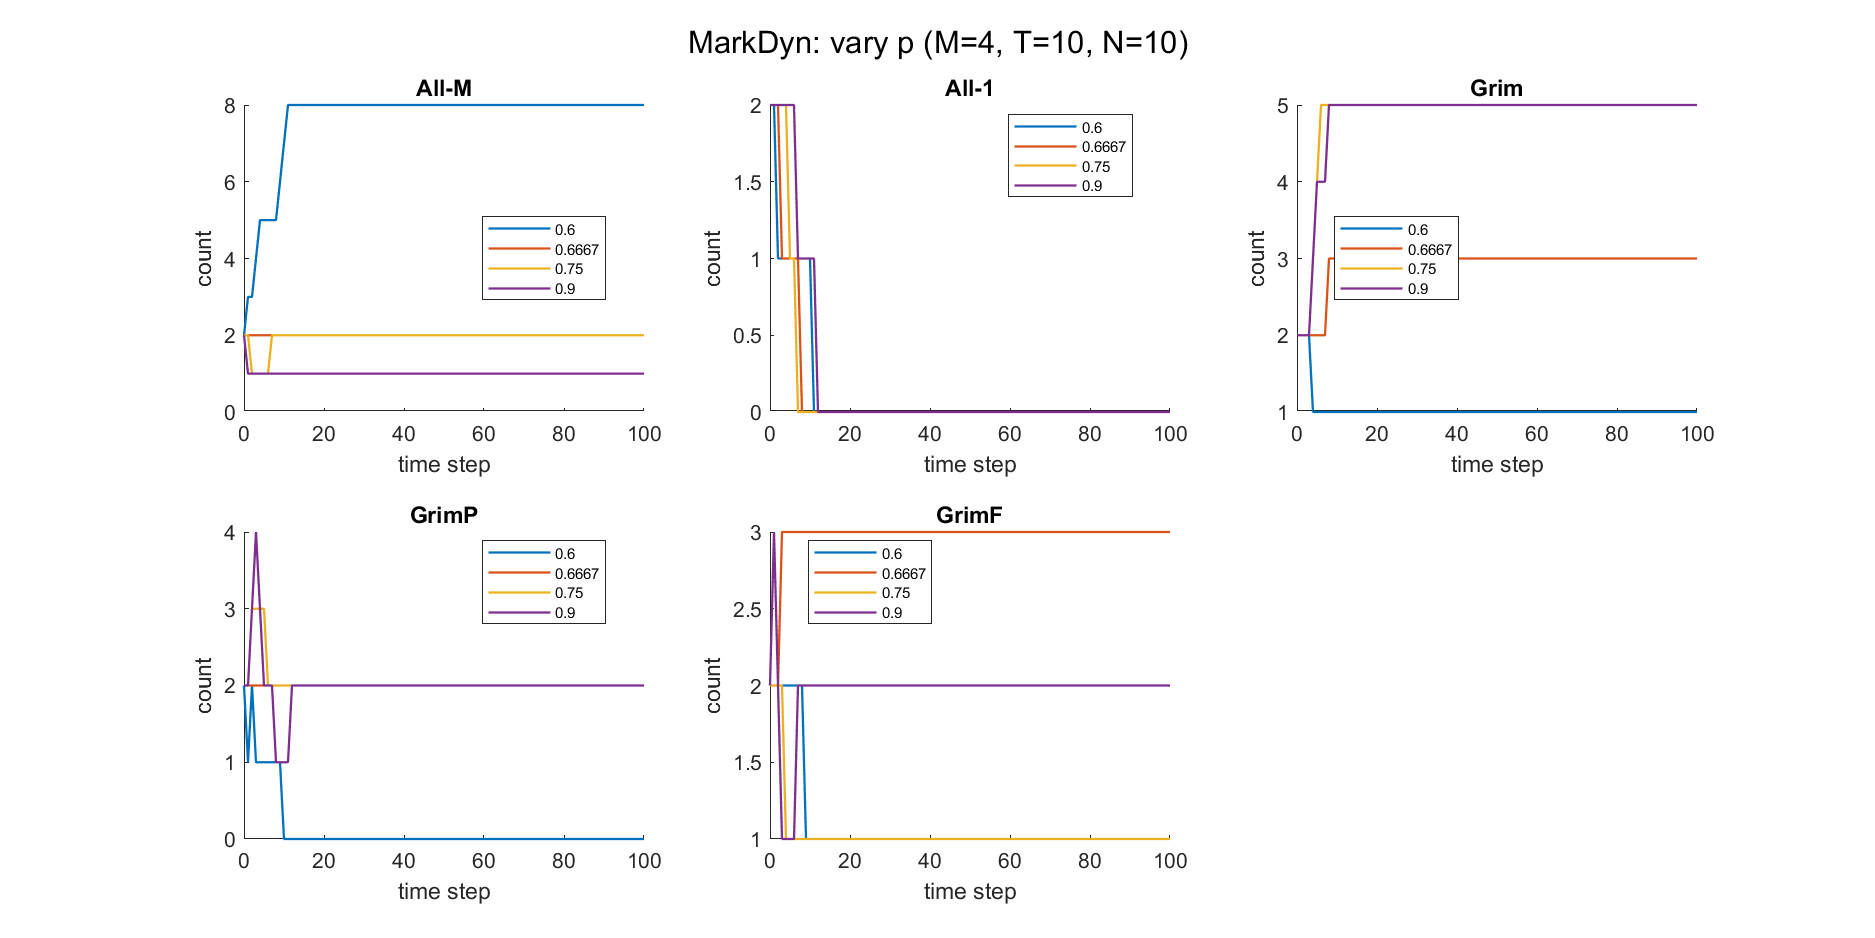
\includegraphics[width=\textwidth]{mark_overlay_vary_p}
  \caption{Effect of $p\in\{3/5,2/3,3/4,9/10\}$ on Markov dynamics ($M=4$, $T=10$, $N=10$).}
  \label{fig:mark_vary_p}
\end{figure}

\begin{figure}[H]
  \centering
  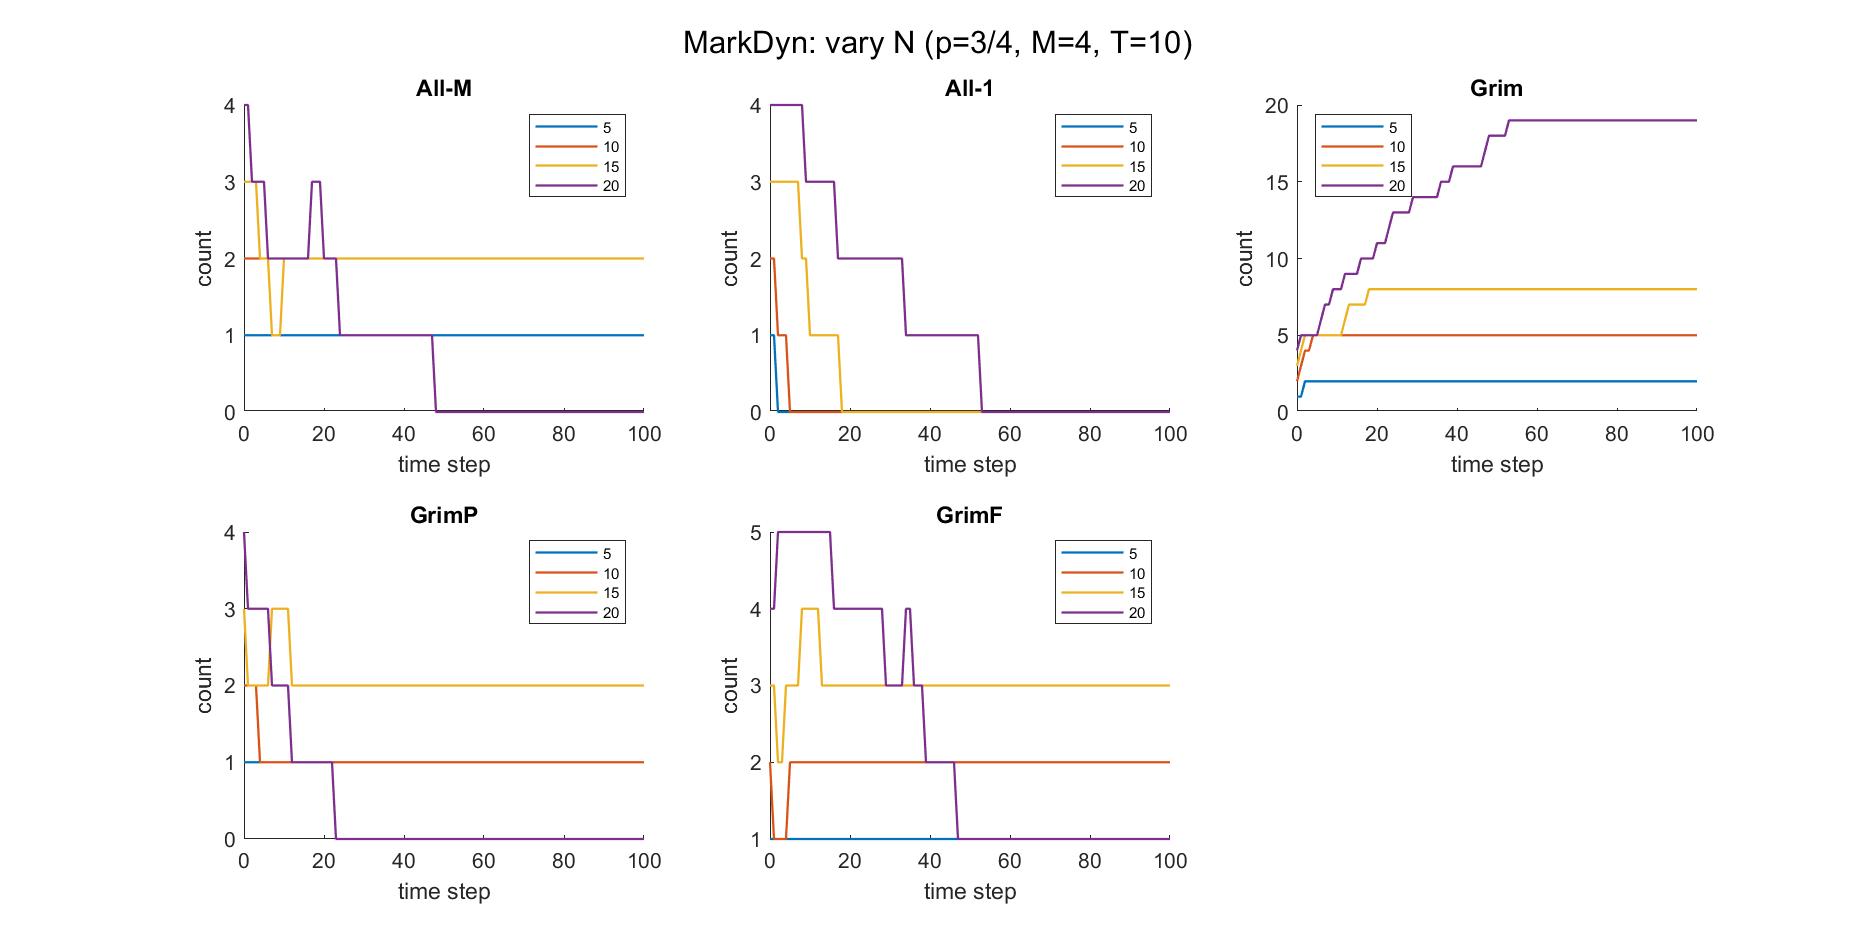
\includegraphics[width=\textwidth]{mark_overlay_vary_N}
  \caption{Effect of $N\in\{5,10,15,20\}$ on Markov dynamics ($p=3/4$, $M=4$, $T=10$).}
  \label{fig:mark_vary_N}
\end{figure}

\begin{figure}[H]
  \centering
  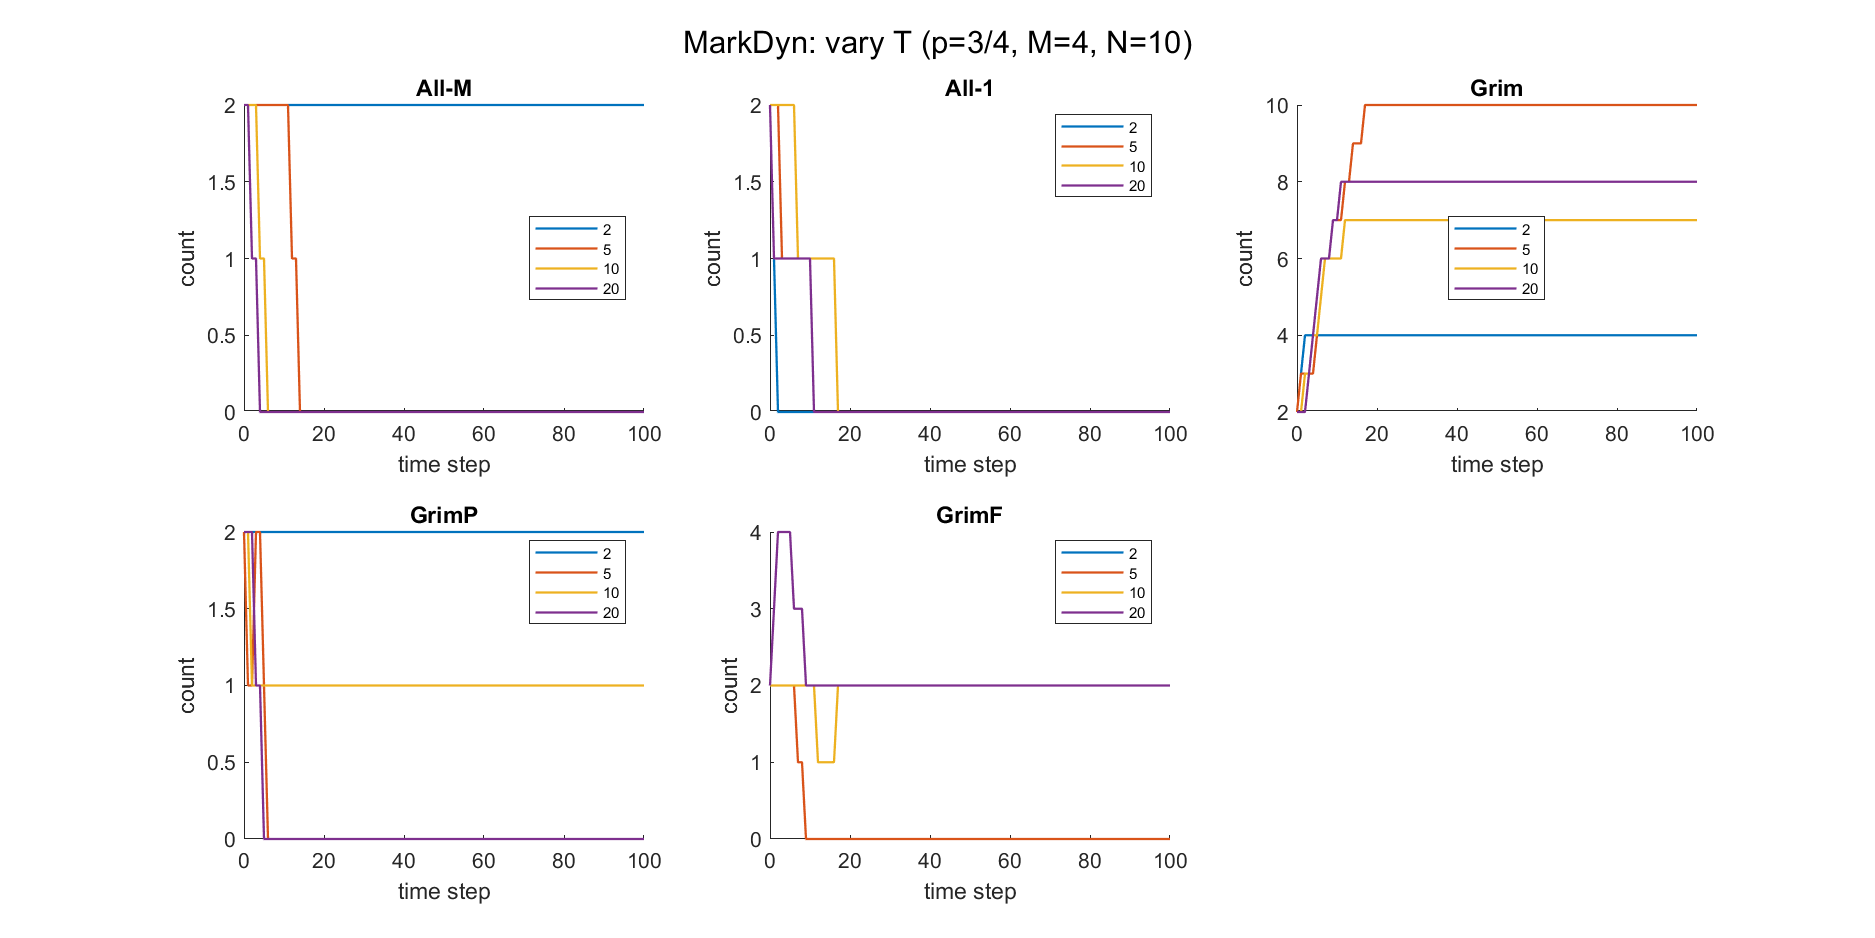
\includegraphics[width=\textwidth]{mark_overlay_vary_T}
  \caption{Effect of $T\in\{2,5,10,20\}$ on Markov dynamics ($p=3/4$, $M=4$, $N=10$).}
  \label{fig:mark_vary_T}
\end{figure}

\begin{figure}[H]
  \centering
  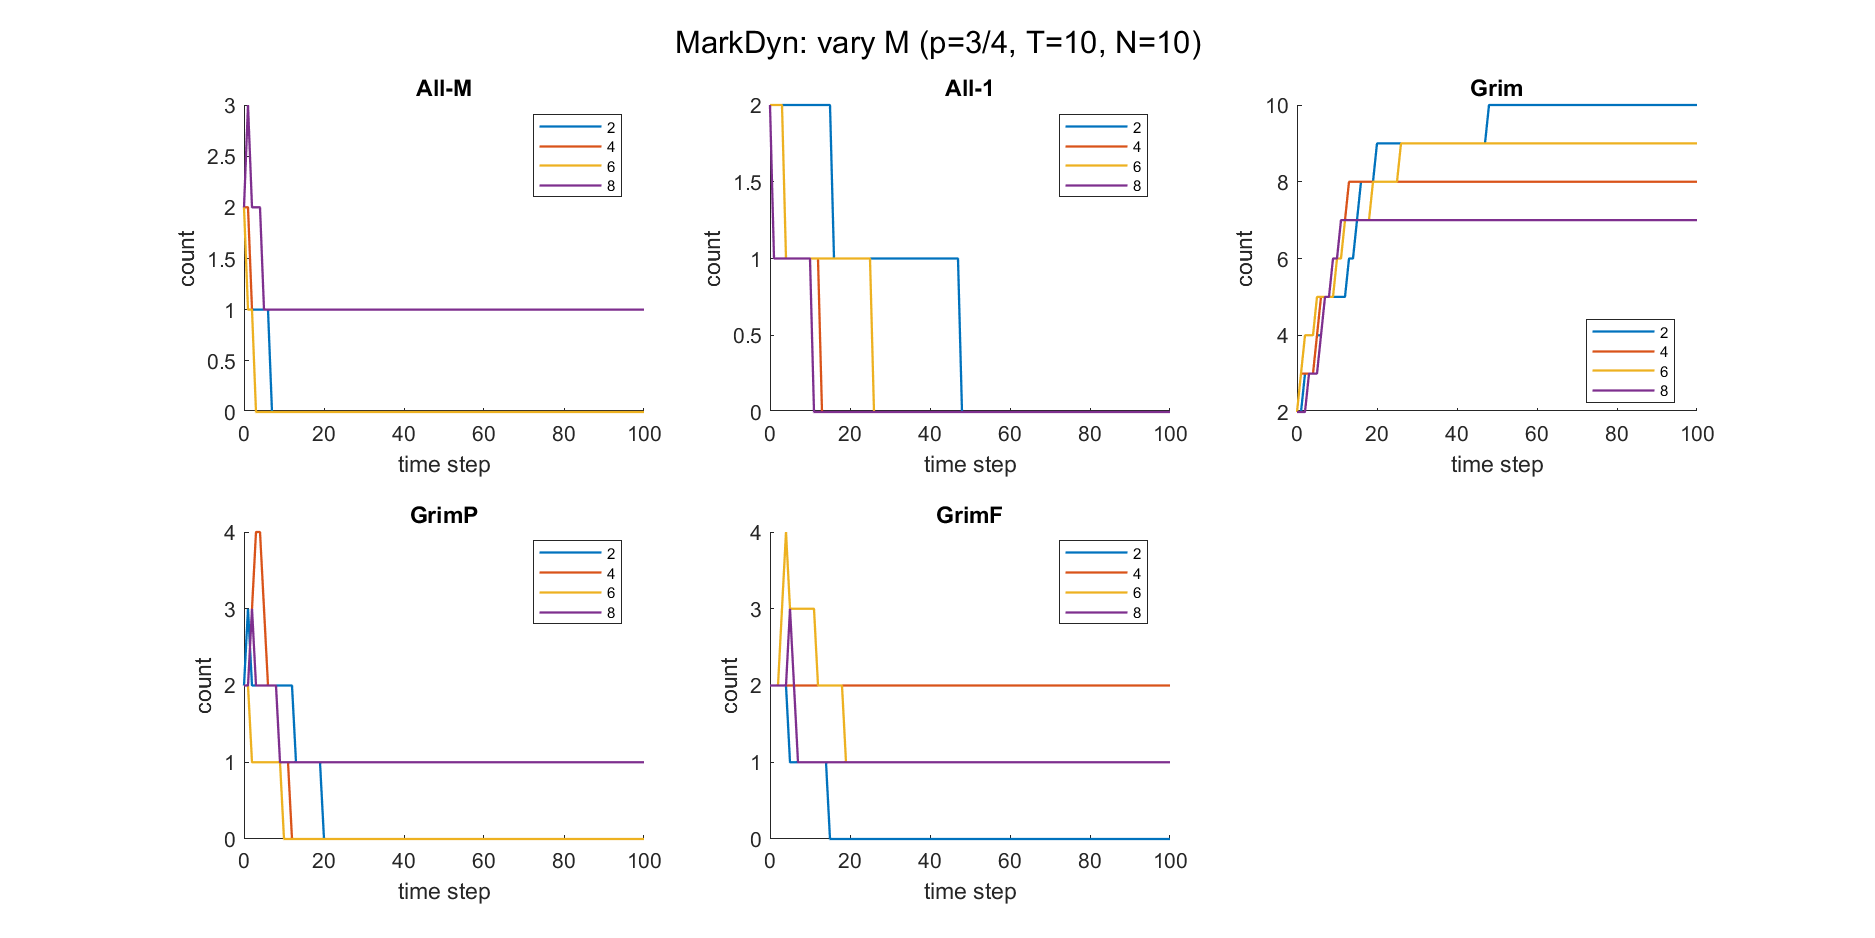
\includegraphics[width=\textwidth]{mark_overlay_vary_M}
  \caption{Effect of $M\in\{2,4,6,8\}$ on Markov dynamics ($p=3/4$, $T=10$, $N=10$).}
  \label{fig:mark_vary_M}
\end{figure}

%============================================================
\section{Connection to Learning Theory}
\label{sec:learning}
%============================================================

Both evolutionary game theory (EGT) and individual learning models describe
adaptive behaviour through the same formal dynamics but under different
interpretations~\cite{BorgersSarin1997,Sandholm2010}.

In EGT, $x_m(t)$ denotes the population share of strategy $m$, and the
replicator dynamic~\eqref{eq:rep} describes how more successful strategies grow.

In a learning model, individual agents update mixed strategies based on
accumulated payoff experience.  Under \emph{reinforcement learning}, the
propensity $q_m$ to play strategy $m$ evolves as
$q_m(t+1)=q_m(t)+\alpha\pi_m(t)$ with $x_m(t)=q_m(t)/\sum_n q_n(t)$.
As shown in~\cite{BorgersSarin1997}, this rule converges in large populations
to the replicator dynamic.

In the five-strategy ISC context this duality has the following interpretation:
\begin{itemize}
  \item \textbf{Evolutionary.}  The four cooperating strategies are
        \emph{evolutionarily neutral} relative to each other (equal fitness
        $TM$ on $\mathcal{F}$).  Natural selection acts only on the
        All-$1$/cooperator axis, with threshold $p^*=2/3$.
  \item \textbf{Learning.}  A rational agent learning from experience will
        reinforce any cooperating strategy over All-$1$ when $p<2/3$, because
        cooperation yields higher average payoff ($TM$ vs $T$).  Among
        cooperating strategies, reinforcement is indifferent (equal payoffs),
        so the agent's internal mix over $\{$All-$M$, Grim, GrimP, GrimF$\}$
        is determined by initial conditions and random variation.
  \item \textbf{Finite-population.}  PPI corresponds to \emph{social learning}:
        agents imitate better-performing neighbours.  The absorbing face
        $\mathcal{A}$ captures the long-run state where social learning has
        eliminated All-$1$ from the population.
\end{itemize}

%============================================================
\section{Conclusion}
\label{sec:conc}
%============================================================

We have studied the Iterated Symmetric Centipede game with five strategies:
All-$M$, All-$1$, Grim, Grim-Patient, and Grim-Forgiver.  The main results are:

\begin{enumerate}
  \item \textbf{Payoff matrix.}  The $5\times5$ ISC payoff matrix $C$
        (Proposition~\ref{prop:Cmatrix}) has a highly degenerate structure:
        all four cooperating strategies earn $TM$ against each other,
        and differ only in their interaction with All-$1$.  Grim-Forgiver is
        the most exploitable: $C(2,5)>C(2,4)>C(2,3)>C(2,2)$.

  \item \textbf{Nash equilibria.}  The ISC has a continuum of Nash equilibria:
        any mixture over $\{$All-$M$, Grim, GrimP, GrimF$\}$ is a NE.
        Additionally, $(\sigma_2,\sigma_2)$ is a NE iff $p\geq 2/3$
        (Propositions~\ref{prop:pureNE} and~\ref{prop:coopset}).

  \item \textbf{Replicator dynamics.}  The cooperative face $\mathcal{F}=\{x_2=0\}$
        is a rest-point set with no internal drift.  The All-$1$ equilibrium
        is stable iff $p>2/3$ (Proposition~\ref{prop:stabA1}).

  \item \textbf{ESS.}  No pure cooperating strategy is an ESS
        (Proposition~\ref{prop:noESS_coop}).  All-$1$ is an ESS iff $p>2/3$
        (Proposition~\ref{prop:ESSA1}).  No mixed strategy in $\mathcal{F}$
        is an ESS (Proposition~\ref{prop:noESS_face}).

  \item \textbf{Markov dynamics.}  The absorbing states form the
        $\binom{N+3}{3}$-element cooperative face $\mathcal{A}=\{s_2=0\}$ plus
        the pure All-$1$ state (Proposition~\ref{prop:absorbing}).
        All states with $s_2\geq 1$ and at least one cooperator are transient.

  \item \textbf{Phase portraits.}  A pentagon projection onto 2-D is introduced
        for visualisation; orbits converge either to the pentagon face
        (cooperative region) or to the All-$1$ vertex.

  \item \textbf{Comparing Grim variants.}  Grim is most resistant to All-$1$
        exploitation; Grim-Forgiver is least resistant but also least
        aggressive (allows partial recovery of cooperation after punishment).
\end{enumerate}

Future work includes: (a) adding Tit-for-Tat and Generous-Tit-for-Tat
strategies; (b) studying the effect of noise/mutation on the neutrally stable
cooperative face; (c) analysing asymmetric populations.

%============================================================
\begin{thebibliography}{10}

\bibitem{Rosenthal1981}
  R.\,W.~Rosenthal (1981).
  ``Games of perfect information, predatory pricing and the chain-store
  paradox.''
  \textit{Journal of Economic Theory}, 25, 92--100.

\bibitem{LK2026}
  I.~Lazaridis and A.~Kehagias (2026).
  \textit{Iterated Symmetric Centipede: Learning and Evolutionary Games}.
  Preprint, March 2026.

\bibitem{Axelrod1981}
  R.~Axelrod and W.\,D.~Hamilton (1981).
  ``The evolution of cooperation.''
  \textit{Science}, 211, 1390--1396.

\bibitem{BorgersSarin1997}
  T.~B\"orgers and R.~Sarin (1997).
  ``Learning through reinforcement and replicator dynamics.''
  \textit{Journal of Economic Theory}, 77, 1--14.

\bibitem{Hofbauer1998}
  J.~Hofbauer and K.~Sigmund (1998).
  \textit{Evolutionary Games and Population Dynamics}.
  Cambridge University Press.

\bibitem{Sandholm2010}
  W.\,H.~Sandholm (2010).
  \textit{Population Games and Evolutionary Dynamics}.
  MIT Press.

\bibitem{Kemeny1969}
  J.\,G.~Kemeny and J.\,L.~Snell (1969).
  \textit{Finite Markov Chains}.
  Van Nostrand, Princeton.

\bibitem{Cressman2003}
  R.~Cressman (2003).
  \textit{Evolutionary Dynamics and Extensive Form Games}.
  MIT Press.

\bibitem{Krockow2016}
  E.\,M.~Krockow, A.\,M.~Colman and B.\,D.~Pulford (2016).
  ``Cooperation in repeated interactions: A systematic review of Centipede
  game experiments, 1992--2016.''
  \textit{European Review of Social Psychology}, 27, 231--282.

\bibitem{SandholmIzquierdo2019}
  W.\,H.~Sandholm, S.\,S.~Izquierdo and L.\,R.~Izquierdo (2019).
  ``Best experienced payoff dynamics and cooperation in the centipede game.''
  \textit{Theoretical Economics}, 14, 1347--1385.

\end{thebibliography}

%============================================================
\appendix
%============================================================

\section{Additional Strategies}

The framework is easily extended.  Further strategies include:

\begin{enumerate}
  \item \textbf{Always-$m$:} always play $\rho_m$ for fixed $m\in\{1,\ldots,M\}$.
  \item \textbf{Tit-for-Tat:} begin with $\rho_M$; in each subsequent round
        play whatever OSC action the opponent used in the previous round.
  \item \textbf{Generous-Tit-for-Tat:} as Tit-for-Tat but forgive defection
        with probability $q=(1-p)/(pM-(1-p))$.
\end{enumerate}

\section{Two-Population Replicator Dynamics}

The one-population replicator dynamics studied in Section~\ref{sec:rep}
necessarily yields symmetric NE.  Non-symmetric NE can be recovered with
two-population dynamics.  Let $\mathbf{x}(t)$ and $\mathbf{y}(t)$ be the
strategy frequency vectors of Population~1 and Population~2 respectively.
The two-population replicator dynamics is:
\begin{align}
  \dot{x}_m &= x_m\left[(C\mathbf{y})_m - \mathbf{x}^\top C\mathbf{y}\right],
  \label{eq:2rep1}\\
  \dot{y}_m &= y_m\left[(C^\top\mathbf{x})_m - \mathbf{y}^\top C^\top\mathbf{x}\right].
  \label{eq:2rep2}
\end{align}
A stability analysis of~\eqref{eq:2rep1}--\eqref{eq:2rep2} for the five-strategy
ISC is left for future work.

\section{Pentagon Barycentric Coordinates}

The pentagon projection maps a frequency vector
$\mathbf{x}=(x_1,\ldots,x_5)\in S_5$ to:
\[
  (X,Y) = \sum_{m=1}^5 x_m\,(\cos\theta_m,\,\sin\theta_m),
  \quad \theta_m = \frac{\pi}{2} - \frac{2\pi(m-1)}{5}.
\]
Key properties:
\begin{itemize}
  \item Pure state $\mathbf{e}_m$ maps to vertex $(\cos\theta_m,\sin\theta_m)$.
  \item Equal mix $(1/5,\ldots,1/5)$ maps to the centroid $(0,0)$.
  \item The cooperative face $\mathcal{F}=\{x_2=0\}$ maps to the convex hull
        of $\{\theta_1,\theta_3,\theta_4,\theta_5\}$, which is the pentagon
        with the All-$1$ vertex removed.
  \item The map is many-to-one: different $\mathbf{x}$ may have the same image.
        Trajectories crossing in the projected space do not necessarily cross
        in the simplex.
\end{itemize}
The MATLAB function \texttt{pentaBary.m} implements this projection.

\end{document}